\documentclass[fr,license=none]{../../../eplsummary}

\usepackage{tikz}
\usepackage{wasysym}

\hypertitle{Philosophie}{2}{FSAB}{1802}
{Beno\^it Legat\and Lucie Mortiaux\and Julien Vaes}
{Stéphane Mercier}

\paragraph{Remarque}
Cette Synthèse a été faite en 2012 et n'est donc pas à jour!
C'est donc un bon complément mais ça ne comprend pas toute la matière.
Si une bonne âme pouvait la mettre à jour, ça serait sympa \smiley.
Par exemple, la partie Logique (qui a été commentée dans le code donc
invisible dans le pdf) n'est je ne pense pas à connaitre
et la partie Bruno Latour n'est pas non plus à connaitre.

\paragraph{Remarque}
Les dates seront notées différemment que le veulent les conventions pour simplifier la lecture.
``IIe siècle ap. J.-C.'' s'écrira donc ``+2s'' et
``Ier-IIe siècles ap. J.-C.'' s'écrira ``+1s,+2s''.
``IIIe millénaire av. J.-C.'' s'écrira ``-3m''.

\part{Ancien testament}
\section{Proche-Orient ancien}
\subsection{Mésopotamie}
\begin{itemize}
  \item Le rite magique;
  \item Faire confiance aux membres de sa famille,
    se méfier des esclaves, ne pas fréquenter les méchants;
  \item Le ``juste souffrant'';
  \item Le mal est la faute de l'homme mais des dieux aussi car c'est
    eux qui ont créé les hommes telles qu'ils sont.
\end{itemize}

\subsection{Égypte pharaonique}
\begin{itemize}
  \item Le monde est ordonné et le pharaon est garant de cet ordre;
  \item Les scribes doivent être vertueux, humble et doivent servir le pharaon,
    ce qui leur promet une prospérité dans ce monde et l'au-delà;
  \item \emph{Instruction de Horjedef}
    La vie après la mort dépend de celle-ci;
  \item \emph{Instructions de Ptahhotep}
    L'ordre social est naturelle et
    assure la permanence de l'ordre cosmique;
  \item \emph{Instructions d'Amenemhat}
    ``juste souffrant'',
    ce n'est par parce qu'on est bon qu'on aura jamais de malheur;
  \item \emph{Instructions d'Amenemope}
    Il faut quand même être bon
    car on sera répompensé par Dieu dans l'au-delà.
\end{itemize}

\section{Le corpus sapientiel}
Le corpus sapientiel est un partie de l'ancien testament contenant 5 livres
\begin{itemize}
  \item Le livre de proverbes;
  \item Le livre de Job;
  \item Le Qohelet ou l'Ecclésiaste;
  \item Le Siracide ou l'Ecclésiastique;
  \item La sagesse de Salomon.
\end{itemize}

Ces livres ont été écrit pas le peuple Juif qui entre les deux premiers
et les 3 derniers se sont éparpillés dans le Proche-Orient notamment en
Grèce ce qui explique la présence de la culture grecque dans les 3 derniers.

\subsection{Proverbes}
\begin{itemize}
  \item Le roi est garant de l'ordre cosmique;
  \item Le monde est ordonnée, il punit les coupables et récompense les justes.
\end{itemize}

\subsection{Job}
\begin{itemize}
  \item Le ``juste souffrant'' apparait.
    On peut aussi souffrir bien qu'on a pas fait de mal.
\end{itemize}

\subsection{Qohelet}
\begin{itemize}
  \item Le discours est attribué à Salomon;
  \item Il remet en cause ce que l'on croit juste et ordonné et la place
    privilégiée de l'homme et la providence qui surveille et punit;
  \item Il ne sombre pas dans le pessimisme mais suggère d'apprendre
    à apprécier la vie jour après jour sans se faire d'illusion sur
    son importance. Carpe Diem en somme;
  \item Contre toute atteinte, il termine par proner la crainte
    de Dieu et le respect de ses commandements.
\end{itemize}

\subsection{Siracide}
Croissement entre culture grecque et juive.
\begin{itemize}
  \item Héritage grec: intellectualisme primé par rapport au travail manuel;
  \item Alliance entre Dieu et les hommes: les hommes ont accès à la sagesse
    de Dieu car ce sont des créatures de Dieu mais les Juifs sont
    dépositaire de la plénitude de cette sagesse;
  \item Le fondement de la sagesse est la crainte respectueuse de Dieu;
  \item La condition d'existence du bien implique la nécessaire
    condition d'existence du mal,
    c'est à dire que le mal est définit dès qu'on définit le bien;
  \item Par contre, l'existence du mal est la responsabilité de l'homme
    et pas de Dieu.
    Le mal est définit mais rien n'oblige l'homme de l'utiliser,
    ce n'est plus la faute de Dieu s'il l'utilise.
\end{itemize}

\subsection{Sagesse de Salomon}
\begin{itemize}
  \item Pogrom sur les juifs, ils veulent donc la quitter pour ne plus
    être juifs et ne plus être persécutés;
  \item Retour à la théodicée traditionnelle;
  \item Le mal est une épreuve que le juste doit surmonter se remettant à Dieu.
\end{itemize}

\part{Le monde gréco-romain}

\section{La différence entre parler et agir}
Il y a une différence entre être philosophe et parler de philosophie.
Le véritable philosophe ne se reconnait pas à son langage mais à sa vie qui révèle le sérieux de sa démarche
(ou qui essaie car une intention qui vise à la droiture sans y parvenir n'est pas méprisable).
La valeur d'un homme ne se mesure pas aux paroles qu'il profère,
mais se laisse entrevoir dans ce qu'il fait de sa vie, jour après jour.

Les penseurs antiques ont été particulièrement attentifs à cette distinction.
\begin{itemize}
	\item Des satiristes comme \textbf{Lucien de Samosate} (+2s) ont ridiculisé les soi-disant philosophes qui,
		en dépit de leurs grands airs et leurs beau discours, se comportaient de façon indigne;
	\item L'éminent biographe et moraliste que fut \textbf{Plutarque de Chéronée} (+1s,+2s),
		dans son œuvre consacrée aux grandes figures de l'Antiquité gréco-romaine,
		a mis l'accent sur les traits quotidiens permettant de voir qui ils étaient vraiment plutôt que sur leurs grands exploits.
	\item Pour \textbf{Cicéron} (-1s), il est indispensable d'unir la théorie à la pratique :
		la théorie doit s'épanouir dans la pratique, sous peine de n'être qu'un discours
		creux, indigne de l'attention d'une personne sérieuse.
		Lui-même s'est d'ailleurs efforcé de
		conjuguer l'excellence intellectuelle à la gestion des affaires en refusant d'isoler la pensée
		de l'action. La \emph{constantia} est à ce prix : la \emph{constantia} est la
		la ``cohérence'' d'une démarche. Il serait absurde de vouloir séparer les deux versants, théorique et pratique
		même s'ils sont distincts.
\end{itemize}

\section{La vertu}
Au fond, une seule question a de l'importance : qu'est-ce qu'une vie réussie ?
C'est là le cœur du questionnement philosophique.
On se penche sur ce qui fait l'homme, ce qui fait sa nature propre.

Les philosophes antiques utilise le mot ``vertu'' avec la signification ``excellence''.
Un homme vertueux est un être humain qui s'est accompli comme être humain.

Pour trouver le bonheur, il faut donc être vertueux, c'est à dire, à être excellement l'être humain qu'on est.
Il faut donc répondre à la question ``Qu'est-ce que l'homme ?''.
Ca rejoint l'injonction que les Grecs avaient écrit sur le temple d'Apollon delphique:
``Connais toi toi-même''.
Pour connaitre les conditions d'excellence d'une chose, il faut pouvoir dire ce que cette chose est.
Par exemple, vous pouvez dire qu'une calculette est un mauvais gsm car vous savez que la nature propre
d'un gsm est de téléphoner et d'envoyer des messages.
Ce qu'une calculette ne sais pas faire.

\section{L'âme}
Nombre de penseurs antiques, à la question ``qu'est-ce que l'homme ?'', vont répondre
que l'homme est homme \emph{par son âme}.
Évitons pourtant un grave malentendu ici : l'âme
s'oppose certes au corps, \emph{mais pas nécessairement comme l'immatériel au matériel}.

En effet, jusqu'au $+2s$, la plupart des philosophes sont matérialistes.
Pour eux, l'âme est matérielle mais invisible pour l'œil (ils la voient un peu comme un gaz).

Attention, un même mot, restitué dans une autre langue ou une autre époque peut cacher différentes idées ou nuances.
Par exemple, le philosophe et poète épicurien latin \textbf{Lucrèce} (-1s) dit ``âme'' pour ``système nerveux central'' et esprit pour les processus chimiques ayant court dans notre cerveau.
Du coup, quand il parle d'âme répandue dans tout le corps et l'esprit situé à un lieu précis du corps, il est tout à fait pertinent.

Il n'y avait que \textbf{Platon} et son disciple \textbf{Aristote} qui disait que l'âme relèvait d'un ordre de réalité irréductible à la matière. Il ne s'agit donc pas d'une matière plus subtile, mais de quelque chose de
radicalement différent.
Mais ces deux penseurs font longtemps figure d'exceptions sur cette question.

Une fois encore, qu'il n'y ait pas de malentendu : un être vivant, précisément parce qu'il
est vivant, possède une âme. ``\^Ame'' veut juste dire: principe qui fait de l'être qu'il anime un
être vivant. Maintenant, une âme n'est pas une autre âme ; et ce sont leurs fonctions qui
distinguent les âmes. On peut discerner trois grands ``types'' d'âme :
\begin{description}
	\item [Végétative]
		Une âme végétative est celle d'un végétal ; elle n'est autre que le principe qui rend raison
		du fait que ce végétal est bien un être vivant et que, à ce titre, il possède les fonctions ``de
		base'' du vivant : nutrition, croissance et reproduction.
	\item [Sensitive]
		Si nous considérons ensuite
		l'animal, nous voyons qu'il possède d'autres fonctions (en plus des fonctions de base susdites, bien entendu), qui relèvent de sa sensibilité et qu'un arbre ne possède pas : vue,
		ouïe, etc.
	\item [Intellectuelle]
		Enfin, à ces fonctions s'ajoute, chez l'homme, une capacité d'abstraction, de
		penser non plus seulement des réalités concrètes individuelles, mais se s'élever à des
		concepts, d'appréhender des notions \emph{universelles} : on parle d'une fonction intellective ou
		intellectuelle.
\end{description}

Si nous revenons à présent à la question ``qu'est-ce que l'homme ?'', nous pouvons, selon l'optique des philosophes antiques, répondre en disant qu'il s'agit d'un vivant dont la \emph{animal (animé) rationnel}.

S'ensuit une conséquence capitale pour la philosophie : si l'homme est ainsi qualifié, la
vertu, l'excellence donc, consiste pour lui à se perfectionner selon cette nature rationnelle
qu'il possède en propre. Autrement dit, \emph{la vertu est raison}.
Une vie humainement réussie
est une vie conforme à ce que dicte la raison, qui fait de nous ce que nous sommes en vérité : des êtres humains, distincts des autres vivants.

Ce point de vue a été développé avec une force
toute particulière par les philosophes stoïciens ; pour eux, non seulement la vertu est raison, mais la réciproque est vraie aussi : la raison est vertu.

\section{Stoïcisme}
Fondée à la fin du -4s par \textbf{Zénon de Citium}, ses plus fameux représentants de l'époque
impériale sont trois personnages remarquables:
\begin{itemize}
	\item \textbf{Sénèque}, précepteur impérial et sénateur romain +1s;
	\item \textbf{Épictète}, ancien esclave et enseignant affranchi +1,+2s;
	\item \textbf{Marc Aurèle}, empereur pendant près de vingt ans +2s.
\end{itemize}

Les Stoïciens font aussi la distinction entre l'âme et le corps tout en restant matérialiste (l'âme est matérielle).
Pour eux, pour être vertueux, il faut s'accomplir soi-même en tant qu'être humain.
C'est à dire suivre sa raison.
L'univers, dans son ensemble, est rationnel à leurs yeux, et tout
s'y déploie d'après une logique totale, providentielle et immanente ; et l'homme est une
partie de ce tout rationnel, qui doit s'efforcer de correspondre à la marche générale de
l'ensemble, sous peine d'être entraîné malgré lui par le cours inéluctable du destin :
comme le dit Sénèque, ``les destins guident ceux qui les suivent, et traînent derrière eux
ceux qui se rebiffent''.

Le plus grand danger sont les passions car elles nous font agir contre notre raison.
Les passions sont ce sur quoi on a pas le contrôle, ce qu'on subit.
Pour les Stoïciens, il ne faut pas seulement l'atténuer, il faut l'\emph{éradiquer}.

Les Stoïciens,
comme d'autres penseurs antiques, sont en ce sens des \emph{intellectualistes}.
Mais cela ne signifie pas que l'homme idéal est un raisonneur enfermé dans sa tour
d'ivoire !
Cela veut seulement dire qu'être vertueux, pour un être humain, consiste à vivre
au niveau de l'intelligence comme expression de la raison. Le mal est donc de l'ordre du
dysfonctionnement de la raison, de l'ignorance. En disant cela, les Stoïciens reprennent
une fameuse affirmation de \textbf{Socrate} -5s, le maître de Platon : nul n'est
délibérément mauvais.

Pour eux, être conscient que quelque chose est bon pour nous et avoir la volonté de le faire, c'est pareil.
Si quelqu'un ne fait pas quelque chose qui est bon pour lui c'est qu'il ne sait pas vraiment que c'est bon pour lui.
Le mal est ignorance, car on ne peut pas connaître ce qui est bon et ne pas le vouloir.
Pour eux donc, la volonté suit l'intelligence,
ce que nous sommes tentés d'appeler ``faiblesse de la volonté''
n'est pas autre chose qu'une faiblesse... de l'intelligence.
Si cette connaissance est véritable et qu'on la fait vraiment
sienne, la volonté sera entraînée par cette intelligence saine, et l'action suivra
la connaissance, de sorte que l'on agira comme on pense.

Ceci s'applique indépendemment du niveau social de l'individu,
on peut très bien être un esclave avec une \^ame libre qu'un roi esclave de sa folie et de ses vices.
D'ailleurs les Stoïciens n'étaient pas contre l'esclavage physique qui était une évidence socioculturelle à l'époque.

L'éthique stoïcienne, exigeante certes mais nullement inhumaine --- que du contraire ! ---, se
présente ainsi comme une dévotion totale à la raison qui réside en tout être humain, et par
laquelle celui-ci peut communier à l'ordre d'un monde dans lequel il a sa place. Les désagréments, les peines et les souffrances, si pénibles soient-ils, ne sont pas des maux,
puisqu'ils n'enchaînent pas ce par quoi nous sommes des hommes, libres et invulnérables
à défaut, peut-être, d'être immortels : notre âme. Être libre, vertueux, et (cela revient au
même) heureux, tout cela est en notre pouvoir et à portée de chacun de nous, pour peu que
nous prenions fermement la décision de l'être.

\section{Résumé}
On reconnait un philosophe par ses actes et non seulement par sa parole.
Être vertueux, c'est mener une vie en accord avec sa nature propre, c'est à dire notre raison.
Selon les stoïciens, on doit se débarrasser des passions folles qui nous font perdre de la liberté à notre raison
et se concentrer sur des passions raisonnables.

La volonté suit l'intelligence donc agir mal c'est une faiblesse de la raison.

\section{Exemples de questions}
\paragraph{En philosophie antique occidentale, on parle volontiers d'âme et de corps ; pour autant, ces termes suggèrent une distinction entre le matériel (sensible) et suprasensible, qui n'est pas toujours pertinente. Expliquez.}
Cette distinction remonte à Platon, que, pour beaucoup de philosophes antiques, l'âme est matérielle, autant que le corps, et qu'ils se distinguent l'un de l'autre par la ``densité'' de cette matière qui les constitue, etc.

\paragraph{Parlez des différents types d'âme, de manière à me dire si, selon ce que pensent les philosophes antiques (en l'occurrence, surtout Aristote, mais je n'ai pas insisté sur ce point dans les notes), les carottes ont une âme.}
Pour les philosophes antiques, ``âme'' veut juste dire: ``principe qui fait de l'être qu'il anime un être vivant''.
Le premier ``type'' d'âme est Végétatif, c'est le principe d'être un être vivant et d'avoir donc les fonctions de base de tout être vivant.
La carotte a une âme quand elle pousse gentiment en terre, grandit en se nourrissant, se reproduit,
avant d'être mise à mort,
cuisinée et dévorée pour votre propre nutrition ou celle de votre lapin,
puisque la fonction végétative de tout vivant implique cette assimilation d'aliments.

\part{Le monde chinois ancien}

Remarque à propos de la translittération du chinois : plusieurs systèmes existent, adaptés
aux langues des érudits qui les ont établis.
Vers le milieu +20s, le gouvernement
chinois a défini le système de transcription pinyin (littéralement ``épeler les sons''), qui a
depuis été largement adopté par la communauté internationale, et que je suivrai donc ici ;
voilà pourquoi il sera question, par exemple, de dao et non de tao, qui est la transcription
dite de l'École Française d'Extrême-Orient.

La notion de ``philosophie'' étant liée, pour partie, à la civilisation grecque au sein de
laquelle elle née, et à la pensée Occidentale, héritière de l'hellénisme, il est délicat
d'employer ce terme sans autre précision pour évoquer les réalités du monde chinois.
Non
que la philosophie soit absente de la Chine, bien entendu, mais tout simplement parce que
la délimitation stricte d'un champ du savoir relevant de la philosophie comme nous la
comprenons (et encore, pas de façon univoque) est étrangère à l'histoire culturelle de
l'Empire du milieu : le terme par lequel on désigne la philosophie en chinois a été forgé
au +19s, et est, du point de vue de la signification, un calque du nom grec : zhexue,
``étude de la sagesse''.

\section{Confucianisme}
Jusque là, ceux que nous appelons philosophes se considéraient plus exactement comme
des pédagogues, des lettrés, dépositaires de la culture.
Confucius, qui vécut au
tournant du -5s, était un de ces lettrés, désireux de revivifier les
valeurs du temps passé.
Pour faire bref, à une époque où le pouvoir central des Zhou ne
jouissait plus que d'une autorité théorique, où la réalité du pouvoir était entre les mains de
grands vassaux et d'une multitude de principautés rivales qui ne cessaient de se faire la
guerre, Confucius souhaitait que l'on réinvestît les vertus des anciens sages et rois de
jadis, qui avaient su apporter au monde chinois sa prospérité et sa paix.

Confucius n'avait donc pas d'ambition proprement novatrice.
Et pourtant : en travaillant à
la restauration des valeurs de l'ancienne aristocratie féodale, il les transforma de
l'intérieur : le modèle du junzi, de ``la personne de qualité'' (comme nous disions
autrefois un ``gentilhomme'') devenait accessible à tout un chacun, indépendamment de son
rang social : une aristocratie du mérite devait prendre le pas sur celle du sang.
Pour devenir
cet homme de bien, la voie royale est l'étude, qu'il faut entendre au sens large
d'``apprentissage'', car il ne s'agit pas tant d'être penché sur ses livres que de développer
sa personnalité morale.
Voilà pourquoi, selon le mot de Confucius, tout le monde a
quelque chose à nous apprendre : les bons nous apprennent à imiter leurs vertus ; les
méchants, à ne pas vouloir leur ressembler.

Les livres, pour autant, ne sont pas exclus --- que du contraire : la tradition confucéenne
accordera une importance capitale à des écrits ``classiques'' (relevant de genre littéraires
variés, un peu comme on trouve, dans la Bible, des écrits poétiques, des livres historiques,
recueils gnomiques, histoires édifiantes, etc.), qui illustrent cette voie (dao, le terme
appartient à la langue courante et n'est pas l'apanage d'une tradition philosophique en
particulier) des anciens rois.
Parmi ces derniers, mentionnons au moins la personnalité de
Shun, figure légendaire de la fin du -3m, qui est exemplaire à plusieurs
égards.
Le père de Shun s'était remarié après la mort de son épouse ; sa nouvelle femme
comme le fils de celle-ci haïssaient le jeune homme, et le vieux père en était venu à
partager, lui aussi, ces sentiments hostiles.
Malgré d'incessantes vexations et même tentatives
d'assassinat, Shun continua de témoigner à son indigne famille une piété filiale
exemplaire, qui le distingua tant et si bien qu'il finit par être désigné pour monter sur le
trône.
Finalement, sa vertu triompha des sentiments contraires des gens de sa famille, qui
revinrent de leurs égarements.

Cette histoire édifiante met en avant deux éléments de première importance.
D'abord, la
piété filiale est la vertu chinoise traditionnelle par excellence, à un degré qui nous stupéfie
(car notre tradition privilégie, en dernière analyse, la justice ; et, si nous honorons la piété
filiale, elle ne constitue pas un absolu).
Ensuite, la vertu (de) telle que la conçoivent les
Chinois relève certes de la catégorie d'excellence, mais surtout, il faut la rapprocher du
``charisme'', d'une sorte d'aura magique qui exerce son influence autour d'elle à la manière
dont un parfum diffuse sa fragrance : Shun n'agit pas directement sur son entourage
pour le transformer, mais se contente de développer la vertu qui doit être la sienne en tant
que fils de la famille ; c'est par elle-même, ensuite, que cette vertu triomphe des mauvais
penchants de l'entourage de Shun, comme la bonne odeur, si elle est suffisamment
``forte'', transforme l'atmosphère du lieu où elle est répandue.

Confucius, dans la droite ligne de cette tradition, estime que le premier devoir d'un bon
gouvernant consiste à ``rectifier les noms'', c'est-à-dire à veiller à ce que
chacun agisse conformément au statut qui le désigne et lui assigne sa place dans la société.
Pour peu que chacun s'occupe d'être excellemment celui qu'il prétend être, l'harmonie
se rétablira d'elle-même.
Le souverain, ses ministres, les pères, leurs fils, tous doivent
connaître la place qui est la leur, sans chercher à obtenir celle qui ne leur revient pas ; s'ils
apprennent à être en vérité ceux qu'ils devraient être --- un véritable souverain est un souverain
qui veille au bien de son peuple ; un véritable serviteur ne cherche pas à évincer
son supérieur, mais l'épaule de toutes ses forces ; etc. ---, le monde connaîtra la paix, et les
barbares eux-mêmes, à ce spectacle, voudront se convertir aux bienfaits de la civilisation.

Parmi les vertus qui font l'homme de bien et qui s'apprennent au contact des hommes et
de l'exemple des anciens sages, distinguons-en deux en particulier : le sens des rites et
l'humanité.
Celle-ci, d'abord, est la vertu suprême : le sinogramme qui la désigne
est formé de la clé de l'homme et du nombre 2, de sorte que,
selon ce que suggère immédiatement la lecture du terme qui la désigne, la vertu
d'humanité est celle qui se donne carrière quand un homme de bien interagit avec ses
semblables ; et de là cette définition (parmi plusieurs autres) qu'en donne Confucius lui-même :
``L'humanité consiste à aimer les gens''.
Naturellement, cette bienveillance
de l'homme de qualité dans ses relations avec les autres hommes ne se déploie
pas de manière anarchique.
Ici interviennent les ``rites'', les convenances et conventions
héritées de la tradition.
Or ces usages, qui concernent aussi bien le protocole
sophistiqué de la cour que la manière de s'habiller ou de se tenir à table au jour le jour,
valent par eux-mêmes : les convenances ne sont pas des normes arbitraires, mais possèdent
une valeur objective et sacrée (même si le terme ne convient pas parfaitement,
puisqu'il suppose une distinction sacré/profane typiquement occidentale), de même que
les préceptes quotidiens qui structurent la vie des Juifs orthodoxes et qu'on peut lire, en
particulier, dans le Lévitique et le Deutéronome, sont sacrés à leurs yeux et régissent les
moindres faits et gestes de leur quotidien.
Ces conventions rituelles, qui concernent tous
les aspects de la vie, ne forment un carcan étouffant que pour l'observateur extérieur, car
ils doivent, chez celui qui apprend à les faire siens, devenir une seconde nature, celle de
l'homme qui se comporte comme un être humain digne de ce nom au regard de la tradition qu'il assume et représente.

Le message de Confucius est ainsi une pédagogie de l'excellence individuelle au service
de la communauté humaine, au sein de laquelle chaque homme a un rôle à jouer à la place
qui lui revient.
Mencius -4s; on dit Mencius, comme Confucius,
est le plus fameux des continuateurs de l'œuvre de moralisation entreprise par
Confucius.
Sa lecture de l'éthique confucéenne se fonde sur un pari :
Mencius veut croire en la bonté de l'homme.
Non que l'homme soit bon dès le départ, mais il possède en lui
les germes de la bonté, des jeunes pousses qui, moyennant des
soins appropriés, deviendront des vertus au sens propre.
Nous ne sommes pas une terre
vierge, mais nous sommes d'entrée de jeu orientés vers la vertu, vers la moralité.
Et nous
parviendrons à ce vers quoi nous porte notre nature, mais seulement à condition
d'entretenir avec soin ces germes, pour les développer sans les négliger ni forcer leur
croissance.
Il est constant, en effet, que celui qui arrose trop ses plantes les noie ; et, selon
le célèbre apologue mencien, le fermier qui, pour accélérer sa récolte ``aida'' les jeunes
pousses à grandir en les tirant impatiemment vers le haut vit périr ses espoirs en même
temps que les germes déracinés...

Ce pari sur la bonté de l'homme s'appuie sur des faits d'expérience qui laissent entrevoir
l'existence, en nous, des premiers commencements de la vertu : supposez que, à
l'occasion d'une promenade, seul, vous aperceviez un enfant risquant de tomber dans un
puits.
Avant même de juger de ce que vous ferez (ou ne ferez pas...) pour l'aider, vous
éprouvez comme un pincement au cœur, qui montre que la compassion n'est pas absente
de votre âme.
Permettrez-vous à ce germe de compassion de devenir progressivement la
vertu d'humanité, ou étoufferez-vous ce premier mouvement de votre âme ? Dans un cas
comme dans l'autre, vous avez ressenti le serrement, qui prouve que vous êtes ``fait'',
naturellement, pour la vertu et la bonté dont cette émotion est un prodrome.
De même,
vous découvrirez que vous êtes fait pour l'équité, le rite ou la convenance sociale, et la
sagesse.
Tout homme, hélas ! ne deviendra pas vertueux (même une terre fertile ne rapporte
rien si un cultivateur incapable ou malveillant la maltraite, si les conditions
extérieures sont déplorables, etc.), mais tout homme est par nature tourné vers ces vertus :
la sainteté est dans l'ordre des choses, alors que la perversité est contre-nature.

Un important corollaire de ce qui précède, c'est que tous les caractères qui signalent une
personne vertueuse, en ce compris, donc, les convenances rituelles et tout ce qui est de
l'ordre du construit dans les rapports humains, tout cela suppose qu'il n'y a pas de rupture
entre la nature et la culture.
La culture, ce n'est rien d'autre que le développement de la nature bien comprise.
D'autres voix se font entendre pourtant, parmi les penseurs chinois,
qui se méfient du construit culturel, et dénoncent le dévoiement ``civilisé'' de la nature:
ce sont notamment les Daoïstes.

\section{Daoïsme}
Il est délicat de parler de ``daoïsme'', car l'emploi d'un vocable unique suggère une
continuité d'école, une communauté de valeurs, etc.
Or, le ``daoïsme'' connaît un grand
nombre de variantes, selon les époques et les auteurs considérés : entre l'alchimiste
préoccupé par le ``raffinement du cinabre'' et la confection d'une drogue d'immortalité, le
stratège se réclamant de Laozi, le mystique et philosophe du langage Zhuangzi, les
prêtres-exorcistes de l'Unité orthodoxe, les disparités sont souvent plus patentes que les
similitudes.
Conservons donc l'étiquette ``daoïste'' en ayant à l'esprit l'extrême diversité
de ce qu'elle recouvre.

Le texte le plus fameux du ``courant'' est le fameux Daodejing, le Classique de la voie et
de la vertu, attribué à Laozi.
Or ce texte n'est probablement pas né du jour au lendemain,
mais résulte plutôt d'une tradition qui a fini par se fixer, peut-être dans le courant du
-4s, durant la période dite des ``Royaumes combattants'' (-5s,-3s,
jusqu'à l'unification sous l'égide de Qin Shi Huangdi, le ``premier auguste empereur
de Qin'').
L'histoire de Laozi, sage fonctionnaire dégoûté par la conduite des
puissants, qui aurait dicté son œuvre avant de partir définitivement vers l'Occident, relève
de la légende.
Mais une légende dont on redira l'importance en évoquant, plus tard,
l'arrivée du bouddhisme en Chine à partir du +1s, sous les Han postérieurs.

Ce court texte en prose rythmée, à la manière d'une mystérieuse incantation qui n'est pas
sans évoquer les ruminations divinatoires des chamans, est probablement le plus traduit
des textes chinois dans le monde occidental.
La cause de son succès ? Son extrême diffusion
dans le monde chinois, assurément, mais aussi son caractère ``crypté'', qui le prête à
une foule d'interprétations : s'agit-il d'un manuel de gouvernance, d'un poème mystique,
d'un traité de stratégie, de métaphysique, d'hygiène, de...
? Un peu de tout cela à la fois,
sans doute, avec cependant deux éléments très clairs : un refus de la course aux honneurs
et de l'activisme prôné par les disciples méritocrates de Mozi (dont nous ne parlerons pas
ici), d'une part, et un rejet du formalisme confucéen, de l'autre.

Laozi recommande de se rendre semblable à l'eau, qui paraît faible, puisqu'elle est
contrainte d'adopter la forme que lui impose ce à quoi elle vient se heurter et qui lui dicte
la configuration à adopter, mais qui, en définitive, l'emporte sur les montagnes elles-mêmes,
puisqu'elle est capable de les creuser.
Cette idée de la force du faible conduit à
tirer profit des ressources, de l'énergie à disposition dans l'univers, plutôt que d'opposer
des intentions personnelles limitées aux choses, et de disperser en vain son énergie propre.
C'est la doctrine du ``non-agir'', que l'on se gardera bien de confondre avec
l'apathie : le non-agir n'est pas l'inertie passive, mais le refus du dirigisme, de la
contrainte intentionnelle et de l'affirmation du moi.
Or rien n'est plus efficace que cette
détermination à accompagner le cours des choses sans chercher à s'affirmer égoïstement.

L'un des plus remarquables penseurs daoïstes, qui vécut au -4s, est Zhuangzi.
Parmi les thèmes récurrents de son œuvre, nous retiendrons en priorité son désintérêt pour les affaires politiques et sa critique du langage.
Tel l'oiseau mythique ne se
nourrissant que d'aliments choisis et dédaignant le rat mort dont se gave un oiseau aux
goûts moins relevés, le sage se moque des fonctions publiques, inutiles et fastidieuses.
Voire extrêmement dangereuses, puisque les trésors que l'on obtient en se mettant au service des puissants sont comme les perles que garde le dragon, et dont on ne se saisit
jamais sans courir un grand risque pour sa vie.
Du reste, la vie à la cour est bien étrangère
à la simplicité naturelle qui convient mieux à l'homme, qui, à l'instar de la tortue, fera
bien de préférer traîner sa queue dans la boue plutôt que de savoir combien sa carapace
sera précieuse, après sa mort, dans le trésor de quelque potentat étranger.

Au fond, quand nous admirons ce qui menace l'équilibre de notre existence, et notre vie
elle-même, nous nous trompons de perspective, nous nous abusons nous-mêmes en ne
comprenant pas la vraie nature de nos besoins.
Ceci relève de l'étude du langage à laquelle se livre Zhuangzi, et qui, pour l'essentiel, revient à affirmer tout ensemble que le
langage est certes un outil précieux (que ce philosophe maniait d'ailleurs en virtuose),
mais que nous avons une fâcheuse tendance à nous laisser éblouir par l'éclat des mots.

Car, au fond, le danger du langage, c'est qu'en disant le monde, il le fige dans des catégories toutes faites, il le découpe, introduisant l'artificiel où il n'a pas sa place.
Plus grave
encore, alors que notre langage reflète notre propre rapport au monde, nous sommes tentés d'absolutiser des catégories relatives, en parlant au nom de l'universel quand nous
n'avons pourtant qu'un point de vue limité sur lui.
À cet égard, nous ressemblons à la
grenouille qui passe sa vie au fond d'un puits, et croit que le monde à sa portée dans ce
puits est le tout de l'univers, et qu'elle connaît le ciel, alors que, si elle sortait seulement
du puits, elle verrait qu'il est infiniment plus vaste que ce qu'elle en avait vu jusque là.

Et quand bien même notre perception serait juste, elle ne le serait que relativement à
nous : dormir dans un endroit humide n'est pas une bonne idée...
indiscutablement, mais
seulement pour un homme ; si le poisson pouvait parler, il dirait le contraire et serait bien
à plaindre s'il devait dormir au sec.
Le bien, l'utile, le beau : ces catégories ne valent que
pour nous, et non dans l'absolu : quand une belle demoiselle se présente, l'homme la regarde tout autrement que le tigre, et le poisson plonge se cacher...
Personne n'a tort dans
cette histoire, sinon celui qui affirmerait que, seul, il a raison.
Bien malin, en effet, celui
qui pourrait dire quelle doit être la référence, la norme d'après laquelle il serait permis de
parler au nom de l'absolu.
Faute de pouvoir adopter un autre point de vue que le nôtre,
voilà que nous raisonnons comme s'il n'en existait pas d'autre ; et si nous pouvions changer, nous ririons sûrement de notre ancienne sottise, comme cette femme qui se désolait
en apprenant qu'elle devait quitter la maison de ses parents pour se marier.
Une fois mariée, pourtant, elle mena la vie de château ; et cette situation aussi agréable qu'inattendue
lui fit prendre conscience de ce que son ancienne frayeur reposait seulement sur
l'ignorance de ce qu'allait être sa condition future.

Dans ces conditions, le mieux que nous puissions faire est d'étendre les limites de notre
perspective, pour essayer de penser par-delà les barrières que nous dressons initialement
en y enfermant notre prétendu savoir.
Nous devons ressembler à cet homme qui acheta un
jour un baume pour soigner les engelures.
L'inventeur avait limité ce baume à son propre
usage, pour se garder de la morsure du froid quand il exerçait son métier de laveur de
soie.
Il crut faire une bonne affaire en vendant la recette, mais l'acquéreur destina le
baume à un usage plus considérable, en soignant les marins de la flotte de son maître, qui
put ainsi mettre en déroute l'armée adverse.
Cette application ingénieuse lui valut de
grandes récompenses, qu'il dut en définitive à sa largeur de vues, puisqu'il avait su adapter à d'autres usages le bien qu'il avait acquis.

C'est là ce que nous devons faire avec le langage : non pas le rejeter en raison des dangers
qu'il recèle, mais tirer parti de ses ressources sans se laisser abuser par lui.
Car les choses ne sont pas toujours ce qu'elles paraissent, ou du moins ne le sont-elles pas assurément,
selon l'apologue célèbre du rêve du papillon : Zhuangzi avait rêvé qu'il était un papillon,
puis il s'éveilla et se rendit compte que cela avait été un rêve...
à moins qu'il ne fût réellement un papillon rêvant seulement qu'il était Zhuangzi ?

Le langage crée un univers artificiel, que l'on doit dominer pour qu'il ne nous domine pas.
Mais cette maîtrise dont parle Zhuangzi n'est pas une mainmise par laquelle l'homme
affirmerait son contrôle sur les choses.
Rejoignant Laozi, il pense que l'homme sage ressemble à de l'eau, et que, loin de chercher à affirmer sa spécificité, ses préférences, ses
intentions, il doit s'oublier en quelque sorte, pour atteindre au ziran, littéralement le ``de
soi-même ainsi'', le spontané.
On comprend que cette spontanéité que vise le philosophe
n'a strictement rien de commun avec le ``cri du cœur'' romantique, puisqu'il s'agit en fait
de s'effacer comme individu pour prendre part à la marche du grand tout sans vouloir
l'insérer de force dans des catégories limitées.
Cette spontanéité est donc celle d'un acquis
devenu une seconde nature, comme l'est l'habileté prodigieuse du grand pianiste dont les
doigts glissent tout naturellement sur les touches de l'instrument.

L'homme accompli est celui qui, par une discipline personnelle que Zhuangzi appelle le
``jeûne du cœur'', a su devenir un miroir où viennent se refléter les choses, suivant une métaphore qui connaîtra un succès considérable, chez les Bouddhistes aussi bien
que chez les néo-Confucianistes à partir des Song, au +11s.

\section{Résumé}

\subsection{Confucianisme}
Pour le Confucianisme, créé par \textbf{Confucius}\footnote{You don't say !}, trois choses sont très importantes:
\begin{enumerate}
	\item Chacun doit être excellemment celui qu'il prétend être.
		Il faut connaitre sa place sans chercher à obtenir celle qui ne nous revient pas.
	\item La culture, c'est à dire les convenances que nos ancêtres avaient trouvés qui nous aident à agir bien.
		Ce n'est pas là des coutumes arbitraires mais bien des convenances objectives.
		C'est pourquoi le Confucianisme apporte une grande importance aux livres et aux écrits.
	\item L'humanité, c'est à dire nos relations avec les gens.
		La culture aide ici à le faire correctement.
\end{enumerate}
C'est donc la pédagogie de l'excellence individuelle au service de la communauté humaine au sein de laquelle chaque homme a un rôle à jouer à la place qui lui revient.

\textbf{Mencius} rajoute que l'homme est bon dès le départ,
il est tourné vers la vertu par nature.
Mais on peut tout autant gâcher cette vertu que l'accomplir.
Comme une plante, il faut l'arroser régulièrement sans la forcer.

La culture doit donc suivre la nature.
Le Daoïsme n'est pas d'accord sur ce dernier point.

\subsection{Daoïsme}
\subparagraph{Attention}
Tous les daoïsmes ne sont pas identiques même s'ils ont le même nom.

La base du daoïsme est un texte de \textbf{Laozi} qui a été très diffusé.
Ce succès vient du fait qu'il prête à beaucoup d'interprétations différentes.
\begin{itemize}
	\item Refus de la courses aux honneurs;
	\item Refus de la méritocratie;
	\item Rejet du formalisme confucéen;
	\item Refus du dirigisme.
		Comme l'eau, il faut laisser la vie suivre son court dans vouloir tout diriger.
\end{itemize}

\textbf{Zhuangzi} rajoute
\begin{itemize}
	\item Désintérêt pour la politique et la cour.
		C'est trop dangereux et loin de la simplicité naturelle qui convient mieux à l'homme.
	\item Critique du langage qui vous fait penser que des perceptions sont absolues alors qu'elle sont relatives.
		Par exemple, ``bien'', ``utile'' et ``beau'' sont relatif à l'homme.
		Il faut étendre les limites de nos perpectives, franchir les barrière dressée par un savoir illusoire.
		Il faut utiliser le langage en tant qu'outil sans se laisser abuser par lui.
\end{itemize}
L'homme accompli est celui qui a su devenir un miroir où viennent se refléter les choses.

\part{Bouddhisme et néo-Confucianisme}

Lorsque nous parlons du Bouddhisme, de quoi parlons-nous ? d'une religion, d'une sagesse ou d'une philosophie ? Une fois encore, nous éprouvons ici les limites de
catégories trop étanches ; et l'on peut d'ailleurs poser la même question à propos du
Christianisme, que certains de ses premiers disciples, aux +2s,+3s en particulier, présentaient volontiers comme une philosophie, puisqu'il s'agit, en vérité, d'aimer
la Sagesse éternelle et incarnée, et que le Christ est le Logos, c'est-à-dire la Raison
même de toutes choses.
Retenons donc ici l'idée, très importante, que, pour être commodes et dotées d'une indiscutable pertinence, les catégories qui nous permettent
d'établir des taxonomies plus ou moins élaborées n'épousent jamais parfaitement les
contours plus subtils des réalités qu'elles s'efforcent de décrire.

Le Bouddhisme propose une vision du monde, plus exactement un ensemble de visions
du monde dont les premiers linéaments remontent à la prédication du Bouddha historique, un contemporain de Confucius (fin -4s-début -5s) qui vécut et
enseigna du côté de ce qui est aujourd'hui la frontière népalaise et dans le Nord de
l'Inde actuelle.

Le choc provoqué par la découverte de ce qu'on s'était efforcé de dissimuler à sa jeunesse dorée --- vieillesse, maladie, mort --- décida celui qui se nommait alors Siddhârtha
Gautama à mener une vie d'ascète itinérant.
S'étant aperçu que les macérations et autres pénitences auxquelles se livraient les ermites, à force d'excès, finissaient par n'être
plus perçues comme des moyens, mais comme des fins en soi, il se concentra tout entier
sur son objectif, ce qui lui permit d'atteindre l'éveil (sk. bodhi, qui signifie exactement
``connaissance, révélation'' de celui qui s'est éveillé au savoir véritable, d'où le nom de
buddha qu'on lui donne --- au passage : dans la suite, la mention ``sk.'' désigne un terme
sanskrit, la langue de l'Inde classique ; et ``p.'', un terme pâli, la langue sacrée du Theravâda, dont nous reparlerons ci-après).
L'enseignement qu'il dispensa alors est
concentré dans ce qu'on appelle le sermon de Bénarès (aujourd'hui VârâNasî, dans
l'Uttar Pradesh, un état du Nord de l'Inde), où il révéla ses quatre ``nobles vérités'' :
\begin{enumerate}
  \item Tout est souffrance,
    c'est-à-dire que toute chose comporte nécessairement
    une part d'insatisfaction, engendre un sentiment de malaise,
    d'incomplétude, de trop ou de trop peu :
    on s'attache à des gens qui nous sont finalement arrachés,
    on vieillit et on meurt,
    on est contraint de se rapprocher de ce que l'on aimerait éviter, etc.
  \item Cette souffrance ne vient pas de nulle part,
    mais est la conséquence imputable à une cause,
    que le Bouddha identifie comme la ``soif'',
    c'est-à-dire le désir d'existence,
    qui nous pousse à investir nos actes d'intentions
    qui en ``alourdissent'' la charge karmique.
    Le karma (sk.), qui signifie simplement ``acte'', désigne plus exactement,
    pourrait-on dire, le code génétique de l'acte,
    c'est-à-dire l'intention qui le constitue comme acte.
    De fait, poser un acte, c'est y injecter un objectif qui le dote
    d'une sorte d'épaisseur et lui confère une certaine densité.
    Cela a des conséquences, qui
    font que l'acte entraîne des effets,
    qui seront à leur tour suivis d'effets subséquents,
    et ainsi de suite, nous entraînant dans la roue du saMsâra (sk.),
    de la transmigration.
    Comprenons bien que cette transmigration qui nous fait renaître
    (plutôt que nous réincarner) n'est pas une chance,
    mais le signe le plus tangible de cette catastrophe qui
    consiste à ne pouvoir échapper à l'enchaînement des vies successives.
  \item Pourtant, cette situation n'est pas une fatalité :
    de même qu'un feu cesse de brûler quand on ne l'alimente plus
    et qu'un effet se dissipe lorsqu'on supprime la cause qui le
    produit, il est possible de supprimer la souffrance en s'attaquant
    à la soif qui l'entraîne, de manière à atteindre le nirvâNa (sk.),
    c'est-à-dire l'extinction.
    La nature exacte de celle-ci est difficile à cerner,
    s'agissant d'un état par définition étranger à tout ce qui est
    doté d'une charge karmique,
    un état d'où est absent toute souffrance,
    puisque tout désir en a été éliminé :
    le nirvâNa est analogue à ce qui se produit lorsqu'une flamme s'éteint.
  \item La quatrième et dernière ``noble vérité'' consiste
    alors à décrire les moyens à mettre
    en œuvre pour atteindre à cette délivrance;
    c'est ce que l'on appelle l'``octuple sentier''.
    Il s'agit de huit éléments de connaissance,
    de discipline morale et mentale qui
    doivent nous permettre d'ouvrir les yeux sur la réalité du monde,
    de manière à comprendre que tout ce à quoi nous nous attachons
    sottement est illusoire et
    cause de souffrance, et, partant, de nous en détacher.
\end{enumerate}
La plus tenace des illusions dont nous devons nous défaire est celle du moi : le Bouddhisme originel insiste sur le fait que ce que j'appelle ``moi'' ne possède pas de réalité
substantielle, dans la mesure où il y a certes des états de conscience, des concepts, des
perceptions, des sensations et des formes physiques qui se succèdent (on les appelle les
``cinq agrégats''), mais rien de tout cela ne peut être ``relié'' à un socle stable, à un
support permanent qui subsisterait ``sous'' les déterminations fluentes.
On peut illustrer
cela en considérant un enfant qui grandit et devient un vieillard : nous avons
l'impression qu'il s'agit d'une même substance durable, affectée de diverses altérations
en un sens périphériques, qui n'entament sont intégrité substantielle ; nous pensons,
pour le dire autrement, que c'est la même et unique personne qui est d'abord un enfant,
ensuite un adulte, et enfin un vieillard.
Pourtant, à tout prendre, on sait aujourd'hui que
pas une seule des cellules qui formaient cet enfant n'est encore présente chez le vieillard : toutes sont mortes à un moment ou à un autre, ont été remplacées, et leurs
remplaçantes ont été remplacées à leur tour, si bien que ce qui nous apparaît comme une
entité stable n'a pas la consistance que nous lui prêtons : la vérité est qu'il n'y a qu'une
universelle fluence.
Il n'y donc a pas de ``je'' ; et ce ``moi'' dont je parle n'est que la
réunion supposée d'états de consciences, d'actes, de concepts, de formes corporelles qui
se succèdent de manière stroboscopique, si l'on peut dire.
En ce sens, le monde est impermanent, et possède un caractère illusoire, non parce qu'il n'existerait pas, mais parce
qu'il est vide, c'est-à-dire privé de toute stabilité.

On comprend par là toute la différence qu'il y a entre le Bouddhisme et son succédané
qui pare de ce nom une forme de psychologie positive où il n'est question que de ``réalisation de soi'' : dans le Bouddhisme, notre principal problème est précisément ce soi
dont il faut apprendre à se défaire ! À cette fin, il nous faut considérer le flux incessant
qui emporte tout et dont on doit se dégager, allégeant ainsi progressivement le fardeau
karmique qui nous est échu, en délaissant la soif d'existence et les illusions attenantes
pour atteindre à la complète délivrance.

C'est là une démarche extrêmement exigeante, et le plus sûr, aux yeux du Bouddha historique, est d'embrasser la voie monastique, de manière à s'efforcer d'éteindre
progressivement le désir à travers nos transmigrations successives.
Finalement, après
des éons d'efforts, on devient un arhat (sk.), définitivement engagé sur la voie qui
conduit à l'extinction : parvenu au terme de son existence, l'arhat ne renaît plus et est
délivré du cycle des transmigrations.

Le Bouddhisme, cependant, se diversifie comme s'est diversifié le Christianisme.
Deux
branches principales vont ``récupérer'' l'enseignement du Bouddha et essaimer en dehors de l'Inde.
Il est remarquable, en effet, de constater qu'après une période où il est en
faveur dans le sous-continent indien (en particulier sous l'empire Maurya, au -3s),
le Bouddhisme reflue et finit par être progressivement évincé, par le Brahmanisme d'abord, et l'Hindouisme ensuite,
si bien qu'il s'épanouit finalement loin des terres qui l'on vu naître.
Il y a d'abord la ``Voie des anciens'', la plus
proche, du point de vue doctrinal, du Bouddhisme originel, qui fleurit dans l'île de
Ceylan (Sri Lanka) et se diffuse, à partir de là, dans toute l'Asie du Sud-Est ; c'est la
forme du Bouddhisme qui, associée à un héritage indien très manifeste, se retrouve donc
en Birmanie, en Thaïlande, au Laos, au Cambodge, dans le Sud du Vietnam, en Indonésie et en Malaisie.

La Bouddhisme Theravâda est contesté par ceux qui le dénigrent comme un ``Petit Véhicule'' en développant de leur côté un ``Grand Véhicule''.
Celui-ci se déplace vers le Nord-Ouest, vers l'Asie centrale ; de là, il se transporte le
long de la route de la soie, jusqu'en Chine, où il s'introduit dès le +1s.
De la Chine, où le Mahâyâna va prospérer, il se diffuse dans l'ensemble du monde sinisé,
c'est-à-dire dans le Nord de l'actuel Vietnam, en Corée et au Japon.
Un des traits caractéristiques qui distinguent le Bouddhisme du Grand Véhicule est qu'il accorde moins
d'importance au salut ``individuel'' (avec la figure de l'arhat), au profit d'un salut
conçu sur le mode de l'entraide grâce au secours apporté par des ``Héros pour l'éveil''
(sk. bodhisattva), qui retardent délibérément leur entrée dans le nirvâna afin de porter
secours à ceux qui peinent sur la voie de l'éveil.
Un bodhisattva est ainsi une quasidivinité bienveillante et secourable qui nous facilite la tâche en contribuant, par sa vertu
propre, à alléger notre fardeau karmique, pour peu qu'on se place sous sa protection.
\begin{center}*\end{center}
Si le Bouddhisme a prospéré en Chine, c'est au départ et dans une certaine mesure sur
base d'un malentendu.
En effet, le Bouddhisme partait avec de sérieux handicaps dans
sa conquête spirituelle du monde chinois : en favorisant la vie monastique, et donc la
retraite hors du monde ainsi que le célibat, il s'opposait directement à des valeurs cardinales de la Chine, à savoir le service rendu au Fils du Ciel et le devoir de piété filiale
(xiao).
Pas de pire crime en effet, dans la société chinoise traditionnelle, que de refuser
de donner une descendance à ses parents, car cela a pour effet de rompre la continuité
des rites familiaux et des devoirs liés au culte des ancêtres.

La méprise consista en ceci : les textes bouddhiques, d'abord peu nombreux, furent traduits en chinois par des érudits qui choisirent de recourir à la terminologie daoïste,
donnant aux lettrés de l'Empire du milieu l'illusion que ces textes bouddhiques étaient
apparentés à ceux de Laozi, et ne relevaient donc pas fondamentalement d'une culture
étrangère.
Or cela cadrait fort bien avec la légende de Laozi quittant la Chine à la fin de
sa vie, allant son chemin vers l'Occident : les textes bouddhiques n'arrivaient-ils pas en
Chine par la route de la soie, c'est-à-dire en provenance de l'Occident ? Cette méprise
initiale favorisa l'implantation du Bouddhisme en Chine à une époque où les intellectuels appréciaient particulièrement l'arrivée sur le marché d'écrits à discuter dans le
cadre de leurs réunions lettrées, en particulier après la chute des Han au début du +3s

Puis, le Bouddhisme, en se diffusant plus largement, apparut progressivement comme
un élément réellement exogène, nettement distinct du Daoïsme.
Mais cela n'advint que
tardivement (+5s,+6s), lorsque les textes bouddhiques avaient déjà solidement
intégré le paysage intellectuel du monde chinois.
La diffusion de plus en plus large de
cette religion étrangère, le succès des penseurs (auprès des lettrés) et des mages bouddhistes (auprès du peuple et des cours semi-barbares qui s'étaient multipliées dans le
Nord de la Chine à cette époque), permirent au Bouddhisme de prospérer, si bien que
des écoles de pensée indiennes purent s'établir en Chine.

Ainsi, par exemple, l'école Mâdhyamika (sk.) de Nâgârjuna (+2s,+3s ?),
dont la doctrine hautement spéculative développait une ``Voie du milieu'' --- ce que signifie le nom de Mâdhyamika --- rejetant le mode de pensée binaire.
Au risque de la
caricature et par souci de brièveté, disons que, pour Nâgârjuna, caractériser les choses
comme simplement vraies ou fausses relève d'une vision simpliste du monde.
Pour faire droit à la doctrine bouddhiste du caractère universellement illusoire/vide des choses tout
en respectant la réalité de notre expérience commune, qui nous donne à voir un monde
non dénué de stabilité, nous devons distinguer deux plans de réalité, deux points de vue
sur le réel : il est vrai de dire que le monde possède une certaine densité, mais c'est une
vérité relative, car cela n'est vrai que du point de vue de l'observateur qui constate pour
lui-même cette consistance dont il dote le monde ; maintenant, à considérer les choses
du point de vue de la vérité absolue, il faut dire que le monde est impermanent et que,
sous l'illusion substantielle, il n'y a que du vide.
Ainsi donc, une même affirmation peut
être à la fois vraie et fausse : vraie du point de vue relatif, et fausse du point de vue absolu ; et inversement.
On comprend par là que le vide dont il est question, et qui
constitue, du point de vue absolu, la nature réelle de toute chose, n'est pas un pur néant :
le néant n'est rien, alors que le vide désigne d'abord la commune impermanence,
l'absence de densité, de stabilité substantielle d'un monde tout entier marqué par le flux
qui l'emporte, sans que rien n'y demeure constant.

Pour Nâgârjuna, donc, ce que nous percevons du monde depuis le point de vue relatif
qui est habituellement le nôtre est comme le voile qui couvre la réalité et en dessine,
pour ainsi dire, la périphérie.
Adopter le point de vue de l'absolu revient alors à ôter ce
voile, pour découvrir ce qui se cache derrière lui : le vide.
Au fond, nous sommes des
rêveurs qui doivent apprendre à s'éveiller du monde onirique où ils sont plongés ; le
rêve (l'univers du relatif) se dissipe alors aux yeux de qui accède au monde tel qu'il est
(l'absolu).
Ce rêve était bel et bien une illusion, non pas au sens où il n'existait pas --- car
c'était bel et bien un rêve ! mais sa consistance se dissipe en regard de la réalité telle
qu'elle est en elle-même.

Pourtant, l'implantation d'un Bouddhisme affirmant son indianité à travers les puissantes métaphysiques des maîtres comme Nâgârjuna, Asanga ou Vasubandhu va se heurter
aux préférences intellectuelles des Chinois.
En forçant le trait, on peut dire en effet que
les Indiens, comme les Grecs, ont une sensibilité plus grande à la philosophie spéculative et à la métaphysique que les Chinois ; ces derniers, à l'instar des Romains, se
sentent plus concernés par l'efficacité ou la mise en œuvre concrète dans la pratique.
Partant, après son arrivée discrète sous le manteau du Daoïsme et une phase de développement subséquent ``à visage découvert'' et durant lequel s'affirme son indianité, le
Bouddhisme va connaître une nouvelle phase d'expansion dans le monde chinois en
s'acculturant, en s'acclimatant à la sensibilité proprement chinoise pour l'efficacité
concrète.
Ce qui va donc se développer en Chine, à partir des +6s,+7s, c'est donc un Bouddhisme revisité ``à la chinoise'', où l'affirmation forte de la
non-substantialité du moi perd une part de sa radicalité, où l'éveil ne doit pas être une
affaire si difficile à atteindre qu'il faut des siècles pour y parvenir, etc.
Une fois encore,
on peut, en caricaturant, dire que le Chinois veut tout, et tout de suite.

Sans nous appesantir ici sur la diversité des écoles bouddhiques chinoises liées au
Grand Véhicule, retenons en particulier le rôle joué par le Bouddhisme Jingtu, c'est-àdire de la ``Terre pure'' : le bouddha Amitâbha (l'un des principaux bouddhas auxquels
se réfère le Mahâyâna, à côté de Siddhârtha Gautama) a préparé pour les fidèles un paradis dit ``de la Terre pure'', où transmigreront leurs âmes pour y œuvrer à leur salut
dans des conditions plus favorables et plus douces que celles qu'ils connaissent dans la
vie présente.
Pour bénéficier de cette transmigration, il suffit de répéter une formule de
confiance exprimant la foi que l'on place dans la compassion de ce Bouddha.
Mieux : le
fidèle bénéficie également du secours direct d'un bodhisattva en particulier, Avalokiteshvara, ``le Seigneur-qui-voit'', et que les Chinois appellent Guanyin.
Ce bienveillant
``Héros pour l'éveil'' joue le rôle d'une divinité secourable, protégeant ceux qui se
confient en lui pour les guider vers le paradis de la Terre pure.
Il est extrêmement intéressant de constater que, sous les Song (+10s,+13s), ce bodhisattva, initialement
représenté sous des traits masculins, a fini par prendre une apparence féminine, devenant ainsi une sorte de mère céleste, dont le rôle n'est pas sans évoquer celui que joue la
très sainte Vierge Marie dans l'économie de la doctrine chrétienne.

L'aspect proprement religieux se manifeste ici plus nettement que l'aspect philosophique, qui était, en revanche, plus nettement appuyé dans le Bouddhisme spéculatif de
Nâgârjuna, par exemple.
Une autre forme de Bouddhisme très marquée par des composantes religieuses, et même plus ou moins superstitieuses, est constituée par un courant
partiellement indépendant du Grand Véhicule, et qu'on appelle le Véhicule de Diamant
(Vajrayâna) : il s'agit du Bouddhisme tibétain, qui s'est développé parallèlement au
Tantrisme indien, avec lequel il est apparenté, avant de se diffuser auprès des Mongols,
puis dans le monde chinois.
Ce Bouddhisme haut en couleurs (assez connu des Occidentaux grâce à la popularité dont bénéficie le Dalaï-lama, chef de la principale école de
cette forme de Bouddhisme), intègre bien des éléments chamaniques dont l'efficacité,
comme la récitation des fameux mantra (sk.), tient au fait même de leur énonciation.

Pour en revenir plus spécifiquement au Bouddhisme tel qu'il se développe dans
l'univers culturel de la Chine, une interprétation volontiers iconoclaste de la doctrine du
Grand Véhicule va connaître un succès prodigieux : le chan, ``méditation'', qui traduit
le sanskrit dhyâna et auquel nous nous référons habituellement sous son nom japonais
de zen (plusieurs termes liés au Bouddhisme nous sont ainsi familiers sous leur forme
japonaise ; cela tient au fait que ce sont des représentants japonais de ces doctrines qui
les ont fait connaître à un large public occidental, en particulier durant la première moitié du +20s).
Une fois encore, sacrifions à la brièveté : le chan radicalise la
doctrine bouddhique relative à l'éveil.
Au fond, de quoi s'agit-il ? De changer son point
de vue sur la réalité, pour découvrir que nous n'avons pas à chercher la vérité ailleurs,
puisqu'elle se trouve toujours déjà là, sous nos yeux.
Le tout est d'apprendre à ouvrir les
yeux pour la voir telle qu'elle est, et non telle que nous sommes habitués à la voir, avec,
s'il est permis de s'exprimer ainsi, les ``lunettes'' de l'illusion.

Il ``suffit'' donc de changer de point de vue.
Les Bouddhistes vont s'interroger sur les
modalités de ce changement, en se demandant s'il advient progressivement (ainsi pensent ceux que l'on appelle ``grad(u)alistes'', pour qui l'éveil se conquiert par degrés, de
même qu'un miroir reflète de plus en plus nettement la réalité qui l'entoure au fur et à
mesure que l'on fait disparaître les taches à sa surface) ou soudainement.
Cette dernière
position est celle des ``subitistes'', qui assurent que l'on parvient à l'éveil d'un seul
coup : le ``miroir'' n'est pas sale, et les seules taches sont celles que l'on imagine.

C'est ce deuxième point de vue qui va s'imposer largement dans le Bouddhisme chan ;
en conséquence, les représentants de ce mouvements rejettent la nécessité absolue de
pratiques ascétiques bien spécifiques, puisque l'éveil peut advenir sans qu'il soit nécessaire de s'entourer d'expédients propres à atteindre graduellement à une prise de
conscience qui consiste, en vérité, à changer tout d'un coup son regard sur le monde.
Pour le dire autrement, la vie monastique n'est pas nécessairement un facteur propre à
nous conduire à l'éveil : celui-ci peut s'atteindre dans une vie extrêmement banale,
puisque la vérité est toujours déjà présente partout et en tout lieu, et qu'on l'atteint non
par une révélation transcendante, mais dès lors qu'on s'y est rendu disponible.

Mais comment se rend-on ainsi ``disponible'' à ce point de vue correct sur le réel ?
Toutes sortes de méthodes sont préconisées, de la plus rude à la plus douce.
Parmi les
plus frappantes (au sens propre...), on peut mentionner celles dont usait Linji, au +9s.
Ce qui nous empêche de voir les choses telles qu'elles sont, ce sont nos habitudes
mentales, les illusions que nous entretenons et dont nous ne parvenons pas à nous défaire, parce que nous les avons profondément intégrées et qu'elles régissent notre mode
de fonctionnement : le seul fait de chercher à s'en défaire relève d'une démarche intentionnelle fondée sur ces évidences acquises qui nous détournent d'un regard simple et
franc sur le monde.
La solution consiste donc à faire perdre pied, à provoquer une manière de commotion mentale pour que, durant un instant, on soit coupé du ``sol'' de ses
représentations habituelles.
Grâce à cet effet de surprise, on se retrouve momentanément
``déconnecté'' d'avec son regard ordinaire sur les choses ; et ce moment peut être
l'occasion d'un nouveau regard porté sur le monde.
Tout est bon, dans ces conditions,
pour provoquer un état de choc qui soit une passerelle vers l'éveil.
Le maître pose une
question...
et surprend le disciple qui réfléchit à une réponse judicieuse en le frappant
inopinément d'un coup de bâton ; le maître formule un discours aussi abominablement
choquant que possible pour déstabiliser son auditeur ; etc.

Tous, naturellement, ne sont pas également partisans d'une telle ``thérapie de choc'' ;
d'autres maîtres chan préconisent en particulier la ``méditation assise'' (ch. zuochan, j.
zazen) : en apprenant à adopter une posture physique et psychique appropriée, nous
pouvons faire le calme en nous pour n'être plus submergés par nos réflexes de fonctionnement habituels.
Pour ``alimenter'' cette méditation, il peut être bon de méditer sur
des réflexions ou questions absurdes (les ``cas juridiques'', ch. gong'an, j. kôan : entre
autres, songer au bruit que fait une main applaudissant seule) et qui, à force d'être tournées et retournées dans tous les sens, épuisent nos habitudes mentales et les conduisent
au point de rupture, qui est alors l'occasion de voir le monde différemment.

\section{Le néo-Confucianisme}
La prospérité du Bouddhisme institutionnel va être durement mise à mal par une persécution de grande envergure déclenchée par le pouvoir central chinois vers le milieu du +9s.
Sous couvert de raisons idéologiques, l'entreprise vise en fait à briser la
puissance temporelle inquiétante des monastères et à accaparer les richesses considérables accumulées par les moines.
Bien que de courte durée, la persécution affaiblit
considérablement l'église bouddhique (le chan, en raison de son lien plus lâche avec
l'institution, est moins affecté) qui, tout en conservant une visibilité et une importance
indiscutables dans l'univers chinois pendant les siècles suivant, perd sa préséance intellectuelle au bénéfice d'un Confucianisme renaissant.

Pourtant, ce retour en force de la pensée de Confucius n'est pas une restitution à
l'identique de l'antique philosophie de l'époque des Royaumes combattants.
En réalité,
le néo-Confucianisme, qui prend son essor au +11s, revendique l'héritage de
Confucius tout en intégrant (plus ou moins consciemment) des éléments bouddhistes et
daoïstes, si bien que Confucius eût été très étonné de voir que l'on professait sous son
nom une doctrine empruntant largement à la métaphysique du Bouddhisme et à la cosmologie spéculative des Daoïstes.
Des emprunts altérés, cela va sans dire, mais qui ne
sont pas concevables indépendamment de l'influence exercée par les doctrines qui les
ont suggérés.
Prenons un exemple : l'idée que toutes choses partagent une commune
nature dans un jeu de renvois aux dimensions cosmiques est clairement tributaire du
Bouddhisme ; la différence est cependant que cette commune nature-du-Bouddha
(``bouddhéité'', en chinois fo-xing) assimilée au vide devient, chez certains néo-Confucianistes, l'omniprésence du principe structurant li, expression d'une singularité
ontologique qui dit l'ordre (métaphysique et moral) des réalités constituant un monde
qui n'a rien d'une illusion impermanente.
De façon plus directement parlante, on peut
aussi évoquer les techniques de ``méditation assise'', largement reprises par les néo-Confucianistes.

Divers penseurs de premiers plan contribuent à ce renouveau confucéen, qui fait ensuite
l'objet d'une synthèse géniale dans l'œuvre de Zhu Xi (1130-1200).
Celui-ci fonde le
progrès moral sur une maîtrise érudite du vaste corpus littéraire dont les Entretiens de
Confucius et le livre de Mencius forment, avec deux traités tirés du Mémoire sur le rites,
le centre de gravité.
L'application dans l'étude doit ainsi soutenir la pénétration intellectuelle des principes moraux qui sont aussi la norme même de l'univers, et conduire le
lettré à la perfection de la sagesse au service de la communauté humaine.

Si Zhu Xi a fait l'objet de vives critiques de son vivant, sa pensée finit par s'imposer,
tant et si bien que sa manière d'envisager la formation de l'élite lettrée devient la norme,
presque sans interruption, depuis le début du +14s jusqu'à la suppression du système des examens, au début du +20s.
L'exercice d'une fonction publique, dans le
monde chinois, passe en effet par un recrutement fondé sur des concours, qui, instaurés
dès les premiers temps de l'Empire, avaient été perfectionnés sous les Tang, au +6s.
Sous les Yuan, au +14s, l'interprétation des Classiques par Zhu Xi devient la
norme de l'orthodoxie confucéenne pour plus d'un demi millénaire.

Mais qui dit concours et examens dit aussi académisme et, à plus ou moins long terme,
sclérose d'une scolastique finissant par tourner à vide.
Pour beaucoup de lettrés, l'accès
à une fonction publique devient alors une fin en soi, le formalisme et le bachotage font
perdre de vue le but véritable de l'éducation lettrée : de fait, l'étude recommandée par
Confucius (et Zhu Xi, s'il est bien compris) n'est pas l'érudition, l'habileté dialectique
ou la virtuosité verbale, mais l'apprentissage de la vie morale, le progrès vers la sagesse.
Ce sera en particulier le rôle de Wang Yang-ming (1472-1529) de le rappeler en critiquant le dévoiement des intellectuels oublieux de l'aspect le plus fondamental de
l'enseignement confucianiste.
Pédagogue, poète, stratège, homme politique et philosophe de génie, Wang développe sa pensée suivant deux axes majeurs qui tiennent en
deux expressions chinoises dont nous allons dire un mot : liangzhi et zhixing heyi.

Liangzhi signifie littéralement ``connaissance du bien'' ; Wang Yang-ming désigne par
là la connaissance morale innée, la conscience morale que possède, selon lui, tout un
chacun, et ce, de façon parfaite et achevée dès l'origine.
Concrètement, tout homme que
je rencontre est un Confucius, un sage.
Naturellement, Wang n'est pas naïf : tout le
monde est très loin de se comporter comme un sage.
Ce qu'il veut dire, c'est que, bien
que nous soyons tous des sages au fond de notre cœur, nous ne le savons pas (une maison peut être alimentée en électricité, il y fait cependant sombre aussi longtemps qu'on
n'y allume pas la lumière) ; aussi le mal dont nous sommes responsables relève-t-il non
pas de notre nature profonde, mais de l'égoïsme qui vient s'interposer entre ce que nous
sommes en vérité et la manière dont nous agissons.
Pour prendre une métaphore parlante, on peut dire que, chaque jour, le soleil brille dans le ciel ; si nous ne le voyons pas,
c'est à cause des nuages qui nous empêchent de le voir.
De façon analogue, notre conscience morale, qui est aussi celle de tout homme, brille dans le ciel de notre xin (cœuresprit, siège de l'activité consciente et de la personnalité morale d'un individu), auquel
elle s'identifie ; si nous agissons mal, c'est que nous laissons ce ciel intérieur se charger
de nuages qui empêchent le bien foncier de s'exprimer.

On voit donc qu'il s'agit d'un pari extrêmement optimiste sur la nature humaine, qui
n'exclut pas, dans le même temps, un constat réaliste de notre misère morale ordinaire.
Cet optimisme foncier se situe explicitement dans la lignée de Mencius ; mais on comprend que la doctrine mencienne a été ``revisitée'' par le Bouddhisme, puisque Mencius
parlait seulement de jeunes pousses, de commencements et de promesses de vertu, et
non pas de vertus d'emblée parfaites, alors que Wang affirme que toutes les vertus se
trouvent toujours déjà à notre disposition, au fond de nous, pour peu que nous dissipions
(ce que ne va pas sans efforts !) les désirs égoïstes qui font obstacle à leur exercice sans
pour cela affecter aucunement leur nature intrinsèque.
Au modèle de développement des
vertus décrit par Mencius se substitue donc un modèle de recouvrement de la vertu sise
dans le cœur-esprit de chaque homme.

À cette conception du sens moral inné s'ajoute la doctrine exprimée par la formule
zhixing heyi, ``unité de la connaissance et de l'action''.
Très simplement, il s'agit de
dire que connaître et agir ne sont que les deux facettes d'une seule et même réalité :
conceptuellement, la connaissance se distingue de l'action (la première est le point de
départ de la seconde ; et la seconde, l'aboutissement de la première), mais elles n'en
sont pas moins liées comme l'avers et le revers d'une pièce de monnaie, l'ubac et l'adret
d'une montagne, deux éléments distincts et cependant indissociables.
Celui qui connaît
véritablement agit en conséquence ; car prétendre connaître sans que cette connaissance
s'accompagne pourtant de l'action appropriée est le signe d'une connaissance superficielle, d'une connaissance indigne de ce nom.
La preuve que vous connaissez la piété
filiale, ce n'est pas de pouvoir réciter le Classique de la piété filiale, mais de mettre
cette vertu en œuvre
\footnote{Pour les cinéphiles, dans Matrix, quand Néo dit à Morpheus
qu'il connaît le kung-fu, celui-ci lui demande de le prouver, non pas en récitant des règles, mais en se mesurant à lui.}.

On retrouve là un élément dont il avait été question à propos de la philosophie antique
occidentale, et notamment chez les Stoïciens, dans la droite ligne de la doctrine socratique selon laquelle ``nul n'est méchant délibérément''.
Inopérante, la connaissance
révèle qu'elle est seulement superficielle.

Wang Yang-ming est ainsi convaincu que le sens véritable de l'étude consiste à recouvrer ce sens moral inné en dissipant les désirs égoïstes, qui obscurcissent notre
connaissance du bien et court-circuitent notre capacité à agir convenablement.
La sincérité n'est pas autre chose, et l'attention respectueuse à l'égard de notre liangzhi
doit nous faire comprendre que toute activité de notre vie est un lieu propre au déploiement de ses ressources.
Un jour, comme un disciple du maître se plaignait de n'avoir
pas le temps de se retirer dans son cabinet d'étude pour se plonger dans les textes classiques et en tirer du profit spirituel, Wang lui expliqua que de tels progrès n'étaient pas
tributaires du temps libre que nous pouvions consacrer aux livres, puisque tout nous doit
nous être bon pour apprendre à en finir avec notre égoïsme : sommes-nous tenus de présider un procès ? Apprenons à ne pas nous irriter, ni juger de façon partisane ; et de
même dans toutes les circonstances de la vie.
Une métaphore illustre cela à merveille:
celui qui se préoccupe trop d'érudition, de composition élégante et de maîtrise théorique
ressemble à un homme qui, voulant se faire cuire du riz, se soucie à ce point de surveiller son feu qu'il en oublie de mettre de l'eau et du riz dans sa casserole.
Au bout d'un
moment, sa casserole vide se fend sous l'action de la chaleur,
et devient inutilisable;
l'infortuné a ainsi dissipé en vain ses efforts,
et --- c'est le cas de le dire ---, il reste sur sa
faim.
Dans le même ordre d'idées, on pourrait dire que celui qui étudie un manuel de
cuisine n'est pas rassasié pour autant ; le manuel n'a de sens que si l'on se met à cuisiner pour de bon.
Et le meilleur cuisinier n'est pas nécessairement celui qui est le plus
expert quand on l'interroge sur les détails de l'ouvrage.
Ainsi en va-t-il de l'étude,
qui est un apprentissage de la vie morale, et dont l'essentiel revient à mettre un terme
aux mouvements égoïstes, de façon à permettre à notre sens moral de répandre sa lumière dans notre vie et dans celle de tous les hommes.

\section{Résumé}
\subsection{Le Bouddhisme}
Le Bouddhisme, créé par Bouddha, enseigne 4 nobles véritées:
\begin{enumerate}
	\item Tout est souffrance.
	\item C'est souffrance est dûe aux fait qu'on porte de
      l'importance aux choses qu'on fait.
      Ça leur donne une charge karmique.
    \item Ce n'est pas une fatalité, il suffit d'arrêter
      de désirer pour supprimer la souffrance.
    \item Il y a 8 éléments, l'``octuple sentier'',
      de connaissance et de discipline morale qui doivent nous permettre
      d'ouvrir les yeux sur le monde et de se rendre compte que ce à
      quoi nous nous attachons est illusoire et cause de souffrance.
\end{enumerate}
La plus tenace des illusions est celle du ``moi''.
Pour le Bouddhisme, ça n'a pas de réalité substancielle.
Ce n'est qu'une succession d'états de conscience \emph{supposé en relation}.

C'est là toute la différence qu'il y a avec le Confucianisme et le Daoïsme où il n'est que question de ``réalisation de soi''.
Dans le Bouddhisme, il faut justement essayer de se défaire de ce ``soi''.

À chaque fois qu'on meurt, on se transfigure en un autre animal.
La seule manière de stopper ce cycle est de devenir un arhat, c'est à dire qu'on a réussi à supprimer tout désir.

Le Bouddhisme s'est diversifié
\begin{itemize}
	\item Bouddhisme Theravâda où il y a une entraide pour atteindre le ``salut''.
		Certains retardent leur entrée au Nirvâna pour porter secours aux autres.
	\item Nâgârjuna rejetait le mode de pensée binaire.
		Dire que le monde n'a pas de réalité substancielle est une vision simpliste des choses.
		Du point de vue relatif, il a une certaine consistance et du point de la véritée absolue, il n'est que vide car impermanent.
	\item En Chine, on s'interresse surtout à comment atteindre l'éveil.
		Il faut donc pouvoir voir cette vérité telle qu'elle est et non comme on la voit.
		Certains bouddhistes vont penser que ce changement de vue est progressif mais dans le Bouddhisme chan, ils vont le voir comme soudain.
		Par exemple, Linji proposait de provoquer une commotion mentale pendant un instant.
		D'autres préconisent des manières plus douces comme méditer sur des questions absurdes.
\end{itemize}

\subsection{Le néo-Confucianisme}
Le Bouddhisme perd de l'influence et le néo-Confucianisme se crée.
\textbf{Wang} développe sa pensée selon 2 axes:
\begin{itemize}
	\item Tout le monde a la conscience morale parfaite dès la naissance mais nous ne le savons pas. L'égoïsme vient donc s'interposer entre ce que nous sommes en vérité et la manière dont nous agissons;
	\item La connaissance et le savoir ne font qu'un.
		Celui qui connait véritablement agit en conséquence, s'il n'agit pas c'est que cette connaissance est superficielle.
		On reconnait ici le Stoïcisme.
\end{itemize}
Il faut recouvrer son sens moral inné en dissipant ses désirs égoïstes qui obscurcissesnt notre connaissance du bien et donc nous empêchent d'agir convenablement.
Il faut aussi ne pas se contenter de la théorie et appliquer nos études en pratique.

\part{Georges Lemaitre}
Il a fait en sorte que l'informatique se développe à Louvain.
Le nom de Georges Lemaitre est moins connu que celui d'Einstein alors qu'il est aussi un pionnier dans plusieurs domaines et qu'il a contredit Einstein, à raison, à plusieurs reprises.

Il nait à Charleroi en 1894 dans une famille bourgeoise.
Il va suivre une formation jésuite au collège du Sacré-Cœur.
Cette formation chez les jésuites lui a appris à être un homme de foi.
Cette formation va être un élément décisif dans sa vie car il apprend que la science et la religion peuvent coexister.
Il ne veut pas faire de passerelle conceptuelle entre les deux.
Il les sépare complètement (autonomie absolue) sans pour autant entrer dans la schizophrénie.
Il ne fait pas d'interprétation théologique des sciences et vice versa.
Par ailleurs, il a en tête que la bible n'est pas un livre de sciences.
Un jour, un professeur jésuite va dire qu'une découverte scientifique est prédis par la bible.
C'est plutôt une malchance selon lui car ca pourrait pousser les gens à faire des ponts entre les prédictions de la bible et les sciences.
Il faut maintenir la parfaite autonomie des deux.

Après les jésuites, on l'a orienté dans les études d'ingénieur des mines à Louvain car la famille avait plusieurs mines.
Il va continuer ses études à Louvain lorsque la guerre éclate en 1914 (20 ans).
Il va s'engager comme volontaire et sera affecté aux soldats qui se battent de front.
Puis il sera nommé dans une escadre d'artillerie.
Il finira la guerre comme adjudant et sera décoré.
Après la guerre il continue ses études qu'il n'aime pas tant que ça, d'ailleurs ses résultats étaient bons mais sans plus.
Mais il se rend compte qu'il préfère les mathématiques et la physique.
Ses résultats qui étaient bons deviennent exceptionnels.
Il est convaincu depuis ses 8 ans que sa vocation est de devenir prêtre.
Son père lui dira qu'avant de rentrer au séminaire, il doit finir ses études.
Il le fait avec plaisir, ce qui lui permet de finir ses études et de rencontrer de très grands scientifiques de l'époque.
Ces rencontres vont l'orienter vers ses domaines de prédilection, soit mécanique classique, relativiste et calcul numérique.
Il va aussi être tenté par le concordisme (jeter des passerelles entre théologie et sciences), il va dès les années 30 être capable de séparer ces deux domaines.
Il va alors finir ses études et faire le séminaire.
La guerre a fait qu'il a du retarder son entrée au séminaire.
Pour ça, ils ont fait un séminaire séparé pour les plus vieux.
Il disposait donc de temps libre beaucoup plus grand et ca va lui permettre de se tenir au courant des évolutions des sciences, d'approfondir ses recherches et donc de travailler à sa formation humaine et scientifique en même temps.

Il va prouver la théorie de la relativité en 1919 en observant une éclipse.
Dans sa formation humaine, il s'intéresse notamment au monde chinois.
Dans ses études au séminaire, il aura sa formation scientifique mais aussi théologique.
Il se sentira bien dans sa formation purement spirituelle de sa formation théologique.
Il va rejoindre une fraternité sacerdotale.
Il tenait vraiment à mener de front ces deux activités mais surtout sans les mélanger.
Il va intégrer plusieurs académies, notamment celle de Bruxelles dont la devise est exactement la philosophie de Lemaitre.
Il proposera un mémoire sur la relativité d'Einstein.
Et obtient une bourse pour allez étudier à Cambridge.
Il va pouvoir développer beaucoup son calcul numérique avec Eddington (scientifique majeur de l'époque).
Il va suggérer à Lemaitre des pistes de recherches capitales dans la suite de ses travaux.
Il obtient d'autres bourses qui lui permettent d'allez aux USA (Doctorat au MIT, Cambridge Massachussetts).
C'est beaucoup de chance car ses différents travaux l'amènent à être au bon endroit au bon moment, là où se font toutes les découvertes scientifiques.
Notamment Hubble, qui découvre que notre galaxie est vraiment très petite par rapport à la taille de l'Univers.
Assez frappé par ces découvertes, il va vouloir faire le tour de plusieurs instituts de cosmologie aux USA.
C'est à ce moment qu'il va élaborer sa théorie sur l'atome primitif.
Dans les années 20, quand il termine sa formation, il va se livrer à un véritable marathon pour être toujours à l'endroit où se font les découvertes.
Il sera alors nommé professeur à Louvain et va être souvent absent pour des séminaires, etc.
Cela fut rendu possible grâce à la bienveillance du recteur qui allégea au maximum son horaire pour lui permettre de continuer ses recherches.

Dans ce cadre, il va développer sa théorie comme quoi l'univers n'est pas statique, il est en expansion.
Il est le principal pionnier de cette théorie.
Il avait beaucoup d'opposants, notamment Einstein.
Le fait que l'univers soit statique, est partagé par la quasi totalité de la communauté scientifique.
C'est pour ca qu'Einstein a fait sa constante cosmologique ``$\lambda$''.
Lemaitre va dire que non seulement il faut conserver cette constante mais qu'en plus, en développant les premiers calculs d'Einstein, on prouve que l'univers est en expansion.
Ça passe assez mal au près des autres.
Au congrès Solvay, il rencontre Einstein qui coupe la conversation car il pense que c'est lié à des concepts théologique et  ne veut rien avoir à faire avec ça.
Lemaitre va insister toute sa vie sur le fait que ça n'a aucun lien.

Lemaitre estime que l'un des corolaires de sa théorie est qu'on ne peut pas concevoir un univers sans commencement à moins de considérer un univers statique.
Notre univers a donc eu un commencement.
Il conçoit un modèle de l'univers où l'entropie est minimale quand on regarde vers le passé.
Il énonce donc la \textbf{théorie de l'atome primitif} (plus tard appelée Big Bang car c'est ainsi que les scientifiques appelaient Georges Lemaitre pour se moquer de sa théorie).
Le problème, c'est que cette question en amène toute une série d'autres sur des caractéristiques de cet atome.
C'est un problème limite car, pour Lemaitre, on ne dispose pas des moyens pour en prouver la réalité, il faut de nouveaux moyens pour prouver la validité de cette théorie.
Notamment parce que ça laisse sous entendre que lors du moment qui précède le déploiement de l'univers, il n'y aurait eu ni espace ni temps ce qui n'a pas de sens au niveau atomique.
L'atome primitif précède l'univers, mais pas du point de vue temporel mais du point de vue logique.
Le temps commence donc avec le commencement de l'univers, après l'atome primitif.
Lemaitre insiste beaucoup, il n'est pas entrain de faire de la théologie de la création.
La théologie de la création ne peut pas récupérer la théorie de l'atome primitif car elle est scientifique, on ne peut pas mélanger les deux!

L'espace temps commence au moment où l'univers se déploie comme on peut le voir sur la Figure~\ref{fig:space_time};
\begin{description}
	\item[$t_1$] 1\ier{} moment d'expansion à vitesse fulgurante
	\item[$t_2$] phase de quasi stabilité
	\item[$t_3$] nouvelle expansion (comme aujourd'hui)
\end{description}
\begin{figure}[!ht]
	\begin{center}
		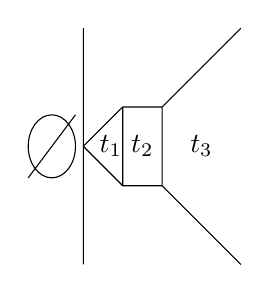
\begin{tikzpicture}[scale=0.5]
			\draw (1, 0) -- (1, 6)
			(1, 3) -- (2, 4)
			--(3, 4) -- (5, 6)
			(1, 3) -- (2, 2)
			--(3, 2) -- (5, 0)
			(2, 2) -- (2, 4)
			(3, 2) -- (3, 4)
			(0.2,3) ellipse (0.6 and 0.8)
			(-0.4, 2.2) -- (0.8, 3.8);
			\node at (1.7, 3) {$t_1$};
			\node at (2.5, 3) {$t_2$};
			\node at (4, 3) {$t_3$};
		\end{tikzpicture}
	\end{center}
	\caption{Espace et temps}
	\label{fig:space_time}
\end{figure}

La physique peut observer le commencement de l'univers, grâce au rayonnement fossile.
Dans les années 30, Georges Lemaitre
fait l'hypothèse de ces rayonnements fossiles/cosmiques (fuite en avant des galaxies car leur spectre lumineux est rouge : elles s'éloignent).
Ce ne fut prouvé qu'après sa mort.
Ces rayonnements sont un peu les hiéroglyphes de l'univers, le premier message de l'univers.
C'est un travail qu'il va faire durant le reste de sa vie, sur l'étude des trajectoires et non la nature de ces rayonnements.
Le modèle de Lemaitre est relativement semblable au modèle d'aujourd'hui, avec quelques différences.
Il estime qu'il y a une expansion à une vitesse fulgurante, puis qui se ralenti.
À ce moment l'univers est quasi stable.
Après un certain temps, l'équilibre va se rompre et l'univers va recommencer à s'étendre.
C'est la situation actuelle.

Ses travaux ne l'empêchent pas de développer sa relation avec les chinois.
Il va d'ailleurs travailler aux relations belgo-chinoises pour que des étudiants chinois puissent venir plus facilement en Belgique.
Beaucoup d'observations vont confirmer les hypothèses de Lemaitre.
Il va donc petit à petit se faire un nom.
Malgré cela, il continue à rester au courant de tout ce qui se passe et il devient assez connu surtout parce qu'en plus d'être un éminent scientifique, il était également prêtre.
Ça va beaucoup intriguer les américains car il est également prêtre catholique.

Einstein va se rendre compte que non seulement Lemaitre a raison mais que ca va l'aider dans ses équations.
Ils vont donc avoir de grandes conversations, surtout sur la constante $\lambda$.
Einstein voudrait la supprimer mais Lemaitre est sur qu'elle existe, il a raison.
Il se fait une réputation.
Il prône toujours qu'entre la foi et la science il n'y a pas de passerelles.
Il va prouver ça notamment dans l'affaire Galilée.
Chacun des partis est en tort car ils ont tout les deux voulu marcher sur les plates bandes des autres.
Lemaitre sera particulièrement content lorsqu'il sera nommé maître dans l'académie pontificale des sciences.
C'est une académie qui doit être excellente du point du vue scientifique mais qui fonctionne indépendamment.
Il sera nommé président de cette académie à la fin de sa vie et va perpétuer cette tradition.
Il va faire des découvertes sans vraiment les prolonger.
Il n'est pas quelqu'un qui veut développer des théories finies, mais progresser et découvrir.
Parmi les domaines dans lesquels il est en avance, c'est notamment les spins up'.
Il va avoir jusqu'à 30 ou 40 années d'avance dans certains domaines.
Il va notamment bien développer les machines à calculer, il est à la pointe de la technologie alors que nous sommes en 1960 (66 ans).
La BurroughsE101, est une machine à calculer exposée durant l'exposition universelle.
Il va vouloir l'acquérir pour l'université, n'hésitant pas à mettre de son propre argent pour l'obtenir.
Cette machine était extrêmement capricieuse.
 A cause de la guerre 40-45 et de l'impossibilité de voyager, il va prendre du retard en matière de physique cosmologique.
Il va donc plutôt s'intéresser aux matières dans lesquelles il n'a pas de retard, à savoir mécanique classique, relativiste (dans une certaine mesure) et le calcul numérique.

Concept de Lemaitre : ``le monde n'est pas obscur, nous avons les capacités de l'explorer et de le comprendre''.
 Il va donc s'intéresser aux trajectoires des rayons cosmiques et non pas leurs compositions.
Lemaitre va pouvoir réaliser des avancées tout à fait remarquables sur le problème des trois corps.
Ainsi que sur un problème de deux corps, la théorie des chocs doubles, là où la force devient infinie.
Il va aussi, au lieu de continuer à disserter sur sa théorie qui est déjà fixée, l'étudier en profondeur.
Notamment sur son atome primitif.
Cela va lui permettre de renforcer le fait que la théologie et la science ne sont pas liées.
Il veut convaincre les deux camps qu'il ne confond pas les deux.

Lemaitre ne va pas beaucoup poursuivre sur la nature philosophique de son atome primitif, car ca ne l'intéresse pas vraiment.
Il pense qu'on est un élément du monde naturel qu'est l'univers et que donc on a les capacités de l'explorer par l'intelligence humaine.
Mais bien qu'il soit explorable, il continue à évoluer.
Il s'opposa à Laplace qui pense qu'il n'y a pas d'incertitudes, Lemaitre pense qu'il y en a.
Elles ne sont pas dues à nos ignorances mais à l'évolution constante de l'univers, notamment au niveau de la physique quantique.
Donc à l'état même de la réalité.

Pour explorer le monde il s'agit de nous faciliter la vie.
Bien que sa théorie ne soit pas accessible à tout le monde.
Il pense qu'on apprend les mathématiques d'une mauvaise façon.
A la place de nous apprendre des trucs dont on n'a pas besoin.
Il va penser qu'on devrait penser comme les machines, afin d'optimiser nos résultats.
C'est une réflexion un peu philosophique.
A la fin de sa vie il va se concentrer sur la simplification d'algorithmes.
Lemaitre n'a pas voulu se focaliser uniquement sur un domaine.
Bien sûr il a de grandes passions.
Mais ses passions ne l'ont pas empêché de s'intéresser à beaucoup d'autres choses, par exemple Molière, le monde Chinois, etc.

Sur son lit de mort, on lui annoncera que le rayonnement fossile à été confirmé expérimentalement peu de temps après il décédera à la suite d'une crise cardiaque.

\part{Thomas Kuhn}
\paragraph{Pour l'examen}
résumer un des deux textes vus et prendre position par rapport aux thèses défendues par l'auteur.

\section{Introduction}
``La structure des révolutions scientifiques'' est un des ouvrages les plus importants du 20\ieme{} siècle.

\subsection{La philosophie des sciences}
\begin{itemize}
	\item Étudie la nature, le développement, les finalités des savoirs scientifiques.
	\item Questionne la notion de vérité dans la connaissance scientifique.
	\item Examine le rapport science/objets qu'elle étudie
	\item Étudie le rapport entre les lois/hypothèses/expérimentations.
	\item Rapport entre les différentes disciplines scientifiques.
	\item Rapport entre les différentes théories à l'intérieur d'une même science.
	\item S'intéresse à la place de la science dans la société.
	\item S'intéresse aux sciences et essaye de dégager certains problèmes, les structures en œuvre dans la pratique scientifique.
\end{itemize}

L'\emph{épistémologie} (épisto = sciences, connaissance), c'est la logique, le raisonnement sur la science.
L'épistémologie a marque la philosophie depuis le début.
En effet, Platon se posait la question ``comment atteindre la vérité ?''.
C'est au 17\ieme{} siècle que vont naître les sciences modernes grâce à Descartes.

Thomas Kuhn est un docteur en physique, un scientifique.
Son ouvrage porte sur le développement des théories scientifiques.
Sa thèse : le développement de la théorie obéit à des révolutions, c'est-à-dire des sauts.
Kuhn se demande, s'il y a une accumulation linéaire de théories, est ce qu'on préserve les acquis précédents ?

\subsection{Conception classique des sciences}
\subsubsection{Temps}
Plus on avance dans le temps, plus la connaissance s'enrichit (accumulation de connaissance).
La science est un progrès continu (surtout au 19\ieme{} et 20\ieme{} siècle) par le \textbf{positivisme} d'Auguste Comte.
Ce courant prétend que la raison va finir par avoir une connaissance absolue en tout.
La raison fera la pleine lumière sur l'ensemble du réel.
On se demande alors : ``comment un tel progrès est-il possible ?''
\subsubsection{Introduction}
La \textbf{théorie scientifique} est constituée d'un ensemble d'hypothèses qui doivent devenir des lois; déduire des choses à partir d'un phénomène observé.
Une loi est généralisable car elle explique toutes les occurrences d'un phénomène et justifie les observations, la prédiction d'un phénomène.
\emph{Mais comment formuler une loi ?} En observant un phénomène plusieurs fois dans différentes situations et en faisant surgir une régularité qui fournira la loi (induction = on part de faits particuliers => lois générales).
Après l'élaboration, on peut apercevoir des conséquences qu'on doit justifier à partir de la loi.
Cette conception de la science est désormais considérée comme déplacée et trop naïve car il suffit d'un contre-exemple pour que tout s'écroule.
\paragraph{Exemples}
\begin{itemize}
	\item \emph{dinde inductiviste} de Rossel (philosophe anglais début 20\ieme{} siècle) : dinde qui se fait nourrir tous les matins à la même heure puis à noël, elle se fait manger => interdit de généraliser à partir se l'expérience.
	\item Mill (philosophe anglais du 19\ieme{} siècle) prouva la même chose avec les cygnes blancs, les cygnes noirs existent donc on ne peut pas généraliser.
\end{itemize}
L'induction ne nous permet pas de fonder une théorie scientifique, l'expérience ne permet pas de valider une théorie (ne garantit pas que les prémisses sont vraies).
\subsection{L'épistémologue Carl Popper ($\pm$ 1930)}
L'ouvrage de Kuhn est une critique de la thèse de Popper.
Sa conception renverse la conception classique ; l'expérience ne peut pas valider une thèse, juste la réfuter.
Il faut falsifier les théories pour trouver les exceptions.
Une théorie qu'on ne sait pas falsifier est alors valide.

Hyp $\Rightarrow$ exp, $\approx$exp, $\approx$hyp (expérience invalide, hypothèse invalide)

Pour Popper, c'est la seule chose qui fonctionne.
Une théorie sera scientifique si elle est réfutable, si elle se confronte à l'expérience et qu'elle s'expose à être réfutée.
Une théorie scientifique cherche à exposer ses points faibles.
Elle peut être tenue pour vraie si elle fournit beaucoup d'occasions pour être réfutée mais ne l'est jamais.
\paragraph{Exemple}
Les anges ont les ailes bleus $\Rightarrow$ pas testable donc pas une théorie // la loi de la gravitation peut être testée, réfutée.
Popper : \emph{La science évolue de manière linéaire, le progrès est expliqué par l'échec et non par la réussite.}
\section{Extraits}
\subsection{Extrait 1}
Les historiens des sciences ont deux tâches : déterminer à quel moment et par qui les lois ont été posées et déterminer les erreurs dues aux superstitions.
Cependant, Kuhn constate que les historiens des sciences ont de plus en plus de mal à reclasser les superstitions, les évolutions...
Cela s'explique par le fait que les théories passées étaient aussi scientifiques que maintenant, pas plus imagées ou mythologiques que les nôtres.
La seule différence entre les théories abandonnées et les théories valides est que les croyances d'avant sont incompatibles avec les nôtres, elles n'obéissent pas à la même structure.
\subsection{Extrait 2}
Pour expliquer, Kuhn introduit la notion de paradigme ; selon lui les ouvrages scientifiques définissent les problèmes scientifiques et les méthodes pour les résoudre.
Ses ouvrages ont été à la base d'accomplissements remarquables, ils permirent une progression car ils ont ouverts des perspectives qui ont convaincu beaucoup de scientifiques d'en faire la base de leur recherche.
D'après Kuhn, ces ouvrages sont des paradigmes.
\subsection{Extrait 3}
Un paradigme est un modèle, un schéma accepté, une sorte de structure inconsciente de la collectivité scientifique au sein de laquelle sont générées les différentes théories.
Cette notion permet d'introduire l'idée de \textbf{science normale : tentative pour forcer la nature à se couler dans la boîte préformée et inflexible que fournit le paradigme
\footnote{C'est la nature qui s'adapte à la science et non l'inverse $\Rightarrow$ \emph{Conception internaliste de la science ; tout se passe \textbf{dans} les sciences.} Ce n'est pas une rencontre entre l'intérieur et l'extérieur, ce sont aux forces de la nature de s'adapter à la théorie scientifique internaliste car il n'y a jamais d'extérieur.
Si on force l'extérieur à rentrer, il n'y a plus d'extérieur.
La théorie est pliée par le réel.}}.
Il explique comment une série de problèmes, méthodes vont devenir majoritaires.
C'est en quelque sorte l'évolution du paradigme.
A sa naissance, un paradigme est \textbf{limité}, au début c'est une \textbf{promesse de succès qui devient ensuite une science normale}.
Les scientifiques vont l'appliquer, le préciser, augmenter la corrélation entre les faits et les prévisions du paradigme.
Ex : théorie de la relativité, le Darwinisme, gravitation...
\subsection{Extrait 4}
Selon lui, parmi les faits étudiés par les scientifiques, ils ne choisissent que ceux qui cadrent avec leurs hypothèses pour réduire la distance entre la théorie et les faits.
(Ex : Galilée a construit ses lunettes pour regarder les astres en connaissant déjà plus ou moins quelle était leur nature.) L'observation est travaillée par la théorie et s'effectue par l'instrument.
Pour Kuhn, la communauté scientifique détermine, par la théorie, quels faits sont significatifs puis démontrent la concordance avec la théorie $\Rightarrow$ cercle vicieux.
L'important est que d'abord le paradigme ne donne que des problèmes dont on peut supposer qu'ils ont une solution.
Seuls ces problèmes  sont dits scientifiques car ils sont compatibles avec les outils que le paradigme fournit.
Les autres problèmes sont rejetés et qualifiés de métaphysiques.

\emph{Méta}\textbf{physique} : historiquement, les ouvrages d'Aristote traitaient de choses au delà.
\emph{Par delà} \textbf{La nature} de la physique (Dieu...) (valable pour tous les êtres alors que la physique étudie les choses dans leurs particularités).
La métaphysique ne peut pas être vérifiée par l'expérience.
\subsection{Extrait 5}
Une fois les problèmes posés, la science normale résout un ensemble d'énigmes (= problèmes posés par le paradigme).
Chaque résolution d'énigme est une confirmation du paradigme donné.
Le paradigme va s'élargir et se spécialiser au fur et à mesure sur des points qui n'ont pas encore été résolus.
Les paradigmes posent les règles, parfois explicitement, qui guident les scientifiques dans leur travail.
D'où l'appellation sciences \textbf{norm}ale (qui posent les normes, les règles).
Des questions de faussetés et de vérités vont se poser.
Un paradigme n'est pas plus vrai qu'un autre, c'est une structure scientifique choisie car il a un succès de progrès plus grand.
Ex : on a choisit le système héliocentrique plutôt que le géocentrique car il explique beaucoup plus de choses.
\subsection{Extrait 6}
Kuhn s'intéresse à l'histoire du paradigme ; comment il a évolué.
Au début, il semble  rendre compte de toutes les observations.
En raison de la spécialisation, de l'amélioration des instruments..., on remarque de plus en plus d'anomalies ; plus on s'intéresse de manière plus précise, plus on va voir ce qui ne va pas.
L'accumulation des ces anomalies et l'incapacité à les résoudre va ouvrir une période de crise du paradigme.
L'échec des normes existantes va pousser la science à en cherche d'autres.
Mais Kuhn dit que les scientifiques sont conservateurs ; ils ne lâchent pas un paradigme comme ça.
Ces anomalies vont d'abord causer une résistance au près de la communauté scientifique.
Il ne suffit pas d'une preuve pour qu'un paradigme soit abandonné (c'est bien car ils n'abandonnent pas à la première difficulté).
Il faut donc qu'il y ait des anomalies ! C'est sur ce point que Kuhn s'oppose à Popper.
La réfutation ne peut pas être le moteur de l'évolution.
Il ne suffit pas qu'un paradigme soit réfuté pour être abandonné.
On peut toujours attribuer la faute à autre chose qu'à la théorie, par exemple : mauvais instrument, erreurs de théories auxiliaires... $\Rightarrow$ \emph{Aucune théorie ne fonctionne toute seule !}
\subsubsection{Exemple de résistance}
La théorie gravitationnelle est un paradigme.
Au 19\ieme{} siècle, la gravitation de Newton est au milieu de la science.
La théorie permet de prévoir l'orbite des planètes.
Mais Uranus ne se trouvait pas où Newton l'avait prédit.
\begin{itemize}
	\item Problèmes d'observation
	\item Instruments précis donc pas possibles que ca soit un problème d'observation
	\item Faute des théories auxiliaires mais pas celle de Newton
	\item Modèle du système solaire erroné ; si Uranus n'est pas à la bonne position c'est qu'une autre planète inconnue se trouve à côté d'elle et l'influence
	\item On a alors découvert Neptune par calculs.
\end{itemize}
\subsubsection{Conclusion}
Jamais la théorie de la gravitation n'a été remise en cause, aucune recherche n'a été effectuée dans le paradigme.
C'est une preuve que la théorie de Popper ne fonctionne pas.
Un paradigme n'est donc jamais abandonné pour des raisons internes même si la crise est grave.
Les scientifiques vont tout faire pour préserver la théorie.
Selon Kuhn, \emph{pour qu'un paradigme soit abandonné, il faut un nouveau paradigme pour le remplacer !} Ex : pour que la théorie de Newton soit abandonnée, il a fallut que celle d'Einstein la remplace.
\subsection{Extrait 7}Il s'agit d'expliquer la relation entre les paradigmes ; deux paradigmes différents ne sont pas compatibles, il n'y a pas de progression continue de l'un à l'autre.
Un nouveau paradigme va remplacer complètement celui qui le précède.
De plus, on ne peut pas comparer objectivement deux paradigmes ; on adhère à l'un ou à l'autre.
Pour un scientifique, le passage de l'un à l'autre est une conversion, un acte de foi.
Ils sont incommensurables car le scientifique, après une révolution, travaille dans un contexte totalement différent de celui avant cette révolution.
Les problèmes sont redéfinis ainsi que les méthodes sur lesquelles ils se concentrent.
Entre deux paradigmes, les normes, les structures de base sont modifiées, elles n'ont plus rien avoir.
Révolutions scientifique, politique déterminent une coupure radicale par rapport à ce qui précède.
\subsubsection{À la place de l'ancien modèle}
C'est la fin d'une révolution lorsque tous les adeptes de l'ancien paradigme sont morts ou sont passés du côté du nouveau.
Il ne s'agit jamais d'une comparaison objective entre deux paradigmes.
Le choix d'un paradigme plutôt qu'un autre se fait selon plusieurs critères : par simplicité, selon les problèmes que l'un peut résoudre et pas l'autre, selon la capacité de mieux s'intégrer, pour des raisons socio-économiques...
En général, il sera choisi  quand il sera plus prometteur.
La promesse de réussite d'un nouveau paradigme ne peut être acceptée qu'en vertu d'un acte de foi.

Une question se pose alors : si la science se développe par coupure, pourquoi perçoit-on l'évolution scientifique comme continue, comme un progrès ?  En science normale, une série d'énigmes progressives dans le cadre d'un même paradigme produit un progrès.
Une fois que la révolution a eu lieu, l'évolution est perçue comme un progrès et les adeptes du nouveau paradigme perçoivent dans l'ancien, les prémisses de leurs propres théories.
Au début d'une nouvelle période, des manuels sont écrits pour poser les bases du nouveau paradigme et ne seront plus remises en cause (passage de paradigme à science normale).
On sauvegarde des idées de l'ancien paradigme et on les englobe dans le nouveau.
Les acquis de l'ancien sont repris de manière différente et ne servant plus à la même chose.
Dans ces manuels, ils reformulent un système sans se soucier de leur émergence (pas d'histoire scientifique).

\section{Conclusion}
Pour Kuhn, s'il y a toujours un progrès à partir de quelque chose, il n'y a jamais de progrès vers quoique ce soit.
De plus, le point de départ d'une phase de progrès est en discontinuité avec la période précédente.
Le développement scientifique n'est pas téléologique ; il n'y a pas d'orientation globale, les paradigmes se succèdent.
Il ne s'agit pas non plus de cumuler un ensemble d'acquis, des expériences objectives ni d'approcher le ``tout'' de la réalité.
A toute révolution correspond l'abandon du paradigme qui le précède.
On ne peut pas faire de la science qu'à l'intérieur d'un paradigme et on n'abandonne pas un paradigme à cause d'une expérience, mais parce qu'un autre arrive.
Le moteur des paradigmes est le conflit entre ceux-ci.

\part{Bruno Latour, politique de la nature}
Bruno Latour se définit comme un anthropologue, un sociologue des sciences et techniques.
À partie cette approche, il va rencontrer plusieurs problèmes philosophiques liés aux sciences et à la politique.

Nous allons analyser son texte comme une introduction en 3 parties :
\begin{itemize}
	\item Description de l'auteur et de ses idées
	\item L'intérêt de son texte
	\item Débat central lié à son œuvre
\end{itemize}

\subsection{Bruno Latour}
C'est un personnage français et atypique dans l'écriture de ses textes.
Il appartient au centre de la sociologie.
C'est un personnage controversé à cause des thèses qu'il défend et à cause de sa perspective qui envisage l'étude des sciences et des techniques à travers la sociologie et l'anthropologie (approche non-scientifique des sciences).
Ses sources d'inspirations sont multiples, atypiques et variées ; ministère de l'environnement, animaux domestiques, dépollution, traitements des déchets… Le thème principal est la question du rapport entre nature et culture/société en remettant en cause cette distinction.
Le point principal : \emph{Ce partage nature/culture est une fiction !} Cette idée est déjà présente dans le texte dès le début :  ``Pourquoi l'écologie politique ne saurait pas conserver la nature ?'' et sciences >< démocratie.
Pour remettre en cause cette distinction, il montre que les sciences sont socialement construites et il essaye de comprendre l'impact des découvertes scientifiques et techniques sur notre manière d'être et leur implication dans notre vie quotidienne.

\subsection{Les sciences sont socialement construites}
Il s'intéresse à comment elles se font au travers d'un ensemble de pratiques et controverses.
Il les inscrit dans le domaine du social et montre que le social donne lieu à la science.
Il tente de rendre compte des conditions sociales dans lesquelles un fait scientifique se produit pour ensuite être oubliées.
Ainsi, ses premières études ont été menées en laboratoire, il étudiait le comportement des scientifiques et leurs instruments.
Il s'inspire de l'ethnographie (description des cultures >< ethnologie qui explique) comme s'il observait un peuple isolé d'Amazonie !

\subsection{Faisant partie intégrante de notre vie quotidienne}
Les objets techniques font partis du monde des hommes.
Ils ne s'opposent pas aux hommes, ils déterminent la vie individuelle.
Il montre que les objets techniques peuvent provoquer certains comportements, les objets inertes provoquent des comportements moraux.
Ex : on voit un dos d'âne, on ralentit.
Ces objets techniques ont quelque chose en eux qui induit un comportement ; ils ne sont donc pas inertes.

Pour résumer, le fait scientifique est considéré à travers un réseau.
La théorie de B.
Latour est donc appelée ;  la théorie de l'acteur-réseau.
Elle prend compte dans son analyse, au-delà des hommes, les objets et le discours, acteurs au même titre que l'homme.
Un objet peut avoir plus d'impacte sur la société que les actions d'un homme.
Ces acteurs sont les nœuds du réseau.
Les conséquences de ce réseau sont de remettre en compte la distinction entre le sujet (agit) et l'objet (subit).
Selon Latour, c'est dans les sciences qu'on peut observer un mélange objet – sujet.

En conclusion, il n'y a que des acteurs ! Pour lui, protéger les sciences et les techniques des objets signifie la disparition des sciences.
Tout comme préserver les sujets moraux des sciences et techniques entrainerait la disparition de ces sujets moraux.
Il dit que les sujets moraux deviennent une fiction si on les écarte de la science ; ils disparaissent car ils sont liés.

\subsection{Thèse centrale}
Le grand partage entre nature et société n'a jamais eu lieu.
C'est une fiction qui se fait passer pour un cadre théorique mais qui en réalité, sert des intérêts politiques.
Il n'y a pas d'un côté une nature objective, universelle et de l'autre des natures subjectives.
Pour argumenter la phrase  ``nous n'avons jamais été modernes'' (cf. texte), Latour commence par un constat : la prolifération des hybrides.
C'est un phénomène qu'on ne peut pas ranger dans les cadres et les disciplines élaborées.
Les hybrides sont des objets dont on ne peut pas dire s'ils appartiennent aux sciences ou à la sociologie (remet en cause les frontières, la question de nature ou de culture).
Pour un phénomène, un débat s'engage : il n'y a plus de distinction entre les secteurs, les domaines (chimie, physique, socio…).
Il va essayer de mettre en avant que, si on confie à un seul domaine, une seule question (politique/ scientifique) ou un problème, on va finir par échouer car la question concerne à la fois le domaine scientifique et politique.
Ex : réchauffement climatique appartient à plusieurs domaines.
Selon Latour, il y a donc toujours une hybridation ; il faut redéfinir le rôle du scientifique et du politicien.
Mais il est nécessaire de comprendre leur complémentarité.
Ce qui le dérange est que les scientifiques se présentent comme des experts dont la position rompt toute discussion.
Ils se sont arrogés au pourvoir ; ils font parler les choses mais font taire les humains ! L'enjeu de l'abandon de cette position est démocratique et donc politique.
Abandonner ce partage entre nature et culture permettrait de mieux faire face aux problèmes écologiques.
[Ex : le protocole de Kyoto : accord entre différents pays pour réduire les pollutions environnementales.
Les scientifiques et les politiciens ont travaillé ensemble sur un même problème.
Ils se sont réunis pour envisager une solution ensemble.]

Pour une meilleure gestion des problèmes environnementaux, il ne faut pas faire entrer la nature en politique mais envisager une forme d'écologie politique qui reprend le rôle de chacun des scientifiques et politiciens.

B. Latour s'intéresse à la place des sciences dans la société.
Il repose certains problèmes d'épistémologie.
[Ex : manière dont une science est découverte et justifiée.] Il y a une proximité entre la démarche de Kuhn et celle de Latour.
Ils insistent tous deux sur la dimension sociale, ils se servent de l'histoire et des controverses basés sur l'existence d'une science unique.
Latour propose d'autres outils de recherche, inspirés de l'ethnographie, et cherche une alternative pratique aux problèmes posés entre culture et nature.
Sa proposition est avant tout politique.
Elle s'intéresse à la composition et au mode d'organisation d'un monde commun.
C'est en ce sens que c'est une démarche d'épistémologie politique.

\subsection{Débats suscités par son texte}
Sa position épistémologique et surtout son rapport tendanciellement relativiste (il n'y a pas de vérité, et donc tout est affaire de croyances).
Continuelle oscillation dans son discours entre une épistémologie relativiste (théorie selon laquelle le moteur des sciences: n'est pas la vérité $\rightarrow$ Kuhn) et une méthodologie relativiste.
On peut penser qu'il essaye de dépasser le gouffre entre réalisme et relativisme.
Relativisme dit que, n'importe qui pourrait avoir raison (crétin et intelligent ont une opinion valable autant l'un que l'autre, leurs opinions ont les mêmes valeurs).
Donc ici pas de relativisme car chaque opinion n'a pas la même valeur.

\section{Extraits}
\begin{enumerate}
	\item pp. 21-28
	\item pp. 31-32
	\item p. 42
	\item p. 47
	\item pp. 55-58
\end{enumerate}

\subsection{Extrait 1}
Il annonce la thèse centrale du premier chapitre ; L'écologie politique ne peut pas conserver la nature, prétendre la représenter en permettant à la nature de faire irruption à la politique car la nature est un obstacle à la parole publique.
Il précise qu'il s'intéresse aux sciences telles qu'elles se font ce qui est différent de s'intéresser au discours de la science.
Il s'agit de voir comment la science agit socialement parlant.
Notre représentation  de la science s'inspire d'une représentation dualiste, dichotomique entre science et société.
À un mondé réel objectif s'oppose un monde belliqueux où  opinions et sentiments sont subjectifs.
Le point de départ est le mythe de la caverne de Platon.

\subsubsection{Mythe de la caverne}

Les hommes sont enchaînés face à un mur dans une caverne.
Ils voient des ombres et ne voient que le reflet des idées, de la réalité, qui leur font dos.
Le rôle du philosophe est de se défaire de ces chaînes pour aller contempler les idées (les essences des choses, accéder au réel), pour après revenir dans la caverne et expliquer aux autres que le vrai monde est derrière eux afin de les libérer.
Platon dit qu'il y a beaucoup de chances que le philosophe se fasse tuer, car les hommes préfèrent voir les reflets.

Selon Latour, c'est le point d'encrage de notre vision selon laquelle il y a une séparation entre le domaine de la vérité (sciences) et le domaine des opinions.
Selon lui, cette représentation dualiste suppose 2 ruptures ;
\begin{itemize}
	\item le savant peut s'arracher à ses chaînes et donc le sortir de la caverne;
	\item une fois qu'il a contemplé la vérité, il peut revenir dans la caverne pour discuter de ce qu'il a vu.
\end{itemize}
Ceux qui défendent cette vision (vérité/monde obscur) justifient cela dans le fait qu'une référence à un au-delà est nécessaire pour mettre fin aux agitations de la vie publique.
D'un coté la société qui est un enfer et de l'autre la science qui a droit à la vérité !

Si on renonce à cette séparation, on tombe dans le relativisme.
Il faut aller chercher la vérité pour résoudre les problèmes.
Le savant va chercher la vérité pour mettre tout le monde d'accord.

Mais Latour remet en question cette double rupture.
Elle n'est en aucun cas fondée sur une enquête empirique, ni sur aucun fait d'observation.
Elle est même contraire à la manière dont les sciences se développent, fonctionnent dans la société.
Les sciences naissent dans le social.
Si le philosophe ne sort jamais de la caverne, à quoi sert un tel modèle ? Cette théorie permet seulement aux scientifiques d'acquérir du pouvoir (selon lui), et ainsi circuler entre l'extérieur et l'intérieur pour faire taire les bavardages.
Ce modèle, implicitement convoqué par  toutes les théories scientifiques, est un modèle politique.
Les scientifiques en s'extrayant du monde social exercent en fait un geste éminemment politique, ils opèrent un geste politique en s'opposant à la société.
Il essaye en fait d'abolir la position de l'expert (il n'y a pas de solution toute faite à un problème).
Toute théorie est construite.

\subsection{Extrait 2}

Latour se défend de considérer la science comme une simple construction sociale.
Il consacre l'abandon général du modèle de la caverne.
Il faut sortir de ce modèle, de cette pensée politique occidentale.
Il faut à partir de cet abandon, repenser un nouveau modèle pour la philosophie politique.

\subsection{Extrait 3}

Selon Latour, une caractéristique principale des crises écologiques est qu'elles ont affaire à ce qu'il appelle des objets chevelus ; c'est-à-dire des objets hybrides.
Ces objets spécifiques ont 4 caractéristiques ;
\begin{itemize}
	\item Pas d'essence bien définie (on ne sait pas vraiment ce qu'ils sont);
	\item La production scientifique, technique et industrielle fait partie de leur définition (liés à l'activité humaine);
	\item Ils ont des connections nombreuses (Liés à diverses problèmes);
	\item L'ensemble de la communauté (scientifique) s'attend à ce que ces objets aient des conséquences sociales.
\end{itemize}
Ces objets chevelus déstabilisent la société, ils jettent la communauté dans une situation d'ignorance et d'incertitude (Ex: origine de la vache folle : est-on sûr ?).
Les crises écologiques portent sur la manière de fabriquer tous les êtres.
Autrement dit, cela met en jeu l'ensemble de la production humaine.
L'ensemble du corps social est incapable de dire une fois pour toute ce qu'est tel ou tel objet, quelle est la solution à tel problème.
L'écologie politique déstabilise la notion de nature.

À la fin de l'extrait, Latour dit  ``Dieu merci la nature va mourir'' car il y a une idée de transcendance de la nature qui empêche la parole publique, la vie sociale.
La nature est une entité indépendante du monde humain.
Il faut donc renoncer à cette transcendance pour pouvoir façonner progressivement un monde commun.
On va fabriquer de nouvelles relations basées sur une nouvelle répartition des pouvoirs.
Pour lui la nature n'existe pas en tant qu'élément séparé.
La nature est dans l'homme et l'homme est dans la nature.
Nature et humanité sont impliquées l'une dans l'autre (au même niveau).

\subsection{Extrait 4}

Il faut sortir du modèle : thèse posée.

Une fois le problème posé, il faut une réponse.
Il propose de remplacer la dualité par une seule entité : le collectif.
Ce qui le caractérise, il admet l'imbrication (le mélange) du social et du naturel, ainsi que le concept d'incertitude (pas de réponse définitive).
En se distinguant de la société, le collectif devient la prémisse d'une meilleure répartition des pouvoirs.

Comme Latour le précise, malgré son emploi au singulier, le terme ne renvoie pas à une unité déjà faite, mais à une procédure pour collecter les associations d'humains et de non-humains.
Le collectif - le réseau principal peut être modifié.
Son rôle sera donc de pouvoir soumettre au débat la manière dont on envisage les éléments du milieu, dire ce qui compte et ce qui ne compte pas.
Il est dans un état de perpétuel débat, qui empêche de prendre pour donné ce qui est institué et de pouvoir remettre en question cette construction, institution.

\subsection{Extrait 5}

Il revient une nouvelle fois sur la démarche.
Cette distinction entre nature et société sert de prise de pouvoir et court-circuite le débat public.
La société est toujours en quête de l'expert, de ceux qui savent.
[Ex : en Italie, le président du conseil est un prof d'université car il est considéré comme l'expert le plus à même pour résoudre les problèmes économiques.] Ce n'est donc pas le problème qui appelle un expert mais la manière dont il se pose.
Il défend le rôle et l'intérêt de la philosophie des sciences.

Dès lors, si on passe au système collectif, on peut distinguer 2 notions du terme  ``social'' ; associé à la société, on peut parler de sociale prison (caverne).
Et de l'autre coté de sociale association (engendre le collectif).

Trois traits distinguent les deux modèles :
\begin{itemize}
	\item Le collectif n'est pas menacé par le recours à une nature objective (plus d'opposition entre les deux).
		Les propriétés des êtres sont toujours remises en compte, on ne brise plus le lien social en faisant appel à la nature car tout est toujours soumis à la discussion.
	\item L'avantage du système collectif est qu'il explique comment fonctionne les sciences, il est plus valable épistémologiquement parlant que l'ancien (on n'a pas besoin de sortir de la caverne).
		Il fait l'économie de cette conversion magique du philosophe (du savant).
		Elle est plus à même d'expliquer réellement le fonctionnement réel des sens.
	\item Chaque fois qu'il y a du nouveau, que l'on découvre des objets, on relance la discussion.
		Et à chaque fois que l'on clôture une discussion, on ne clôture jamais l'ensemble du monde commun, il y a toujours de nouveaux débats possibles.
\end{itemize}
Ce système est basé sur le système d'expansion ; toujours débattre sur de nouveaux sujets sans que le débat ne soit jamais clôturé.
Selon Latour, il y a donc une nouvelle répartition des pouvoirs.
Le scientifique est le porte-parole des objets non-humains et non plus UN expert.

\end{document}
\part{La logique}
\paragraph{Pour l'examen}
Expliquer une phrase, en faire la table de vérité et la traduire en langage propositionnel.

\textbf{La logique} vient du grec du grec logos, qui signifie la raison, la logos est la science de la raison.
C'est la sciences qui étudie les règles que doivent respecter tout raisonnement valide.
Elle vient a émergé à l'époque de la Grèce antique, Aristote.
Il explique la logique dans le ``ORGANON''.
Pour lui avant de faire de la logique il faut expliquer la manière de raisonner.
Qu'est ce qu'un raisonnement scientifique.
Le syocisme, ..............
La logique est l outil essentiel pour le raisonnement.
C'est avec le mathémathicien Frege donne une nouvelle vision mathématique de la philosophie.
Il développe deux logique.
D'une part la logique des proposition et de l'autre la logique des prédicats.
Il va raisonner non pas sur des phrases mais sur des symboles.
La logique propositionnel est la logique ou on étudie  la relation entre des proposition, et ces relations vont être combinées ensemble a l'aide de connecteurs logiques:
\begin{itemize}
    \item Négation
    \item Conjonction
    \item Disjonction
    \item Implication
    \item Équivalence
\end{itemize}
\paragraph{Exercice}
On parle de quelqu'un dont on dit ``il aime les fraises et la chantilly''.

Si on se tient au langage courant, il est complexe de se mettre d'accord car il dissimule la logique. L'une des premières étapes de la logique est la simplification.

Une \textbf{proposition} est une affirmation, une phrase déclarative (ex: il pleut).
Cependant toute affirmation n'est pas une proposition.
Une affirmation est une proposition si elle susceptible d'être complètement vrai ou complètement faux (ex: ``je ments'' ).
Prend proposition qui prend en compte un état de fait, met de cote les phrases obtative, impérative ou interrogative.
La logique propositionnelle suit le principe du tiers exclu: un proposition est vrai ou faux pas pas autre choses.
La valeur de vérité d'une proposition est vrai ou faux.
On symbolise une proposition par une lettre ($p,q,\dots$
Dans le cas ou il n y a qu'une proposition, on appelle cela une formule atomique, ce la forme la plus simple du raisonnement.
Si il y a plusieurs propositions on parle de formule composée, c'est là qu'interviennent les connecteurs logiques.Considérons deux proposition $p$ et $q$, on imagine que de $p$ on peut déduire $q$.
``Si $p$ alors $q$'', mais cette phrase peut elle même être vrai ou fausse.
Quand nous combinons des propositions entre elle on obtient une phrase qui elle même à le choix entre deux valeurs de vérité.
La valeurs de vérité d'une formule complexe dépend des formules atomiques qui la compose.

\section{Le connecteur de négation ``$\lnot$''}
C'est le plus simple de tous. Considérons la proposition $p$ et la proposition $-p$ (non $p$).
\begin{center}
    \begin{tabular}{|c|c|}
        \hline
        $p$&$\lnot p$\\
        \hline
        1&0\\
        \hline
        0&1\\
        \hline
    \end{tabular}
\end{center}
C'est une phrase affirmative.
\section{Conjonction: ``$\land$''}
\begin{center}
    \begin{tabular}{|c|c|c|}
        \hline
        $p$&$q$&$p \land q$\\
        \hline
        1&1&1\\
        \hline
        0&1&0\\
        \hline
        1&0&0\\
        \hline
        0&0&0\\
        \hline
    \end{tabular}
\end{center}
Le seul cas ou c'est vrai c'est quand les deux sont vrais.
Il n 'y a pas que le terme ``et'' dans le langage mais aussi ``mais'',$...$.
Il faut donc retrouver les formules atomiques, repérer les connecteurs.
La négation est un connecteur logique, il faut donc toujours la faire sortir.

\section{Exercices}
\begin{enumerate}
    \item ``Pierre et Marie se baignent''\\
        $p$ Pierre se baigne\\
        $q$ Marie se baigne \\
        Connecteur : et\\
        Formule: $p \land q$
    \item ``Pierre et Marie se parlent''\\
        Se parle soit entre eux, soit chacun de leur cÙté.
    \item ``Pierre aime Marie mais ce n'est pas réciproque''\\
        $p$: P aime Marie.
        $q$ Marie aime Pierre.\\
        $p \land (\lnot q)$
    \item ``Il est faux que Pierre aime Marie mais que ce ne soit pas réciproque'' \\
        $p$: Pierre aime Marie.
        $q$: Marie aime Pierre.\\
        A la base: $-(p \land (-q))$\\
        $(\lnot p) \lor q$
    \item ``Pierre n'aime ni le poisson ni le fromage''\\
        $p$: Pierre aime le poisson.
        $q$: Pierre aime le fromage\\
        $(\lnot p) \land (\lnot q)$
\end{enumerate}

\section{Disjonction}
il y a deux types de disjonction:
\begin{itemize}
    \item inclusive(``$\lor$''): vrai si l'un ou l'autre est vraie.\\
        \begin{center}
            \begin{tabular}{|c|c||c|}
                \hline
                $p$&$q$& $p \lor q$\\
                \hline
                1&1&1\\
                \hline
                0&1&1\\
                \hline
                1&0&1\\
                \hline
                0&0&0\\
                \hline
            \end{tabular}
        \end{center}
    \item exclusive (``$\oplus$''): fausse si les deux sont vrais.\\
        \begin{center}
            \begin{tabular}{|c|c||c|}
                \hline
                $p$&$q$&$p \oplus q$\\
                \hline
                1&1&0\\
                \hline
                0&1&1\\
                \hline
                1&0&1\\
                \hline
                0&0&0\\
                \hline
            \end{tabular}
        \end{center}
\end{itemize}
La différence ente les deux ``ou'' se fait en fonction du sens des propositions.
Il faut voir si il y a un lien  ou non.
\section{Implication ``$\Rightarrow$''}
Enoncé du type: ``Si $p$ alors $q$''.
Le seule cas où la proposition est fausse c'est quand a première est fausse.
Si on a l'antécédent faux alors le conséquent es faux.
Condition suffisante (``Si $...$ alors $...$'').
\begin{center}
    \begin{tabular}{|c|c||c|}
        \hline
        $p$&$q$&$p \Rightarrow q$\\
        \hline
        1&1&1\\
        \hline
        0&1&0\\
        \hline
        1&0&1\\
        \hline
        0&0&1\\
        \hline
    \end{tabular}
\end{center}
\section{équivalence ``$\Leftrightarrow$'' ou ``$\equiv$''}
Les deux propositions ont la même valeur de vérité. Ici c'est un condition nécessaire (``ssi''). Interdépendence.
\begin{center}
    \begin{tabular}{|c|c||c|}
        \hline
        $p$&$q$&$p \Leftrightarrow q$ ou $p \equiv q$\\
        \hline
        1&1&1\\
        \hline
        0&1&0\\
        \hline
        1&0&0\\
        \hline
        0&0&1\\
        \hline
    \end{tabular}
\end{center}
\section{Tautologie}
C'est une raisonnement, une formule composée, qui est valide quelque soit les valeurs atomiques qui la compose.
\begin{center}
    \begin{tabular}{|c|c||c|}
        \hline
        $p$&$-q$&$p \lor \lnot q$\\
        \hline
        1&0&1\\
        \hline
        0&1&1\\
        \hline
    \end{tabular}
\end{center}
Ce n'est pas intéressant car c'est toujours vrai, on ne peut pas vérifier quelque choses d'empirique dessus.
Neutre, C'est par l'expérience que l'on peut savoir si c'est vrai ou pas. La logique est quelque chose d'essentiel pour raisonner, mais à c'est limites (contradiction et tautologie).
\section{Execices}
\begin{enumerate}
    \item ``Albert est chez lui ou la lumière n'est pas allumée''\\
        $p$: Albert est chez lui. $q$:  la lumière est allumée\\
        $p \lor \lnot q$
    \item ``Si Albert est chez lui alors la lumière est allumée.'' \\
        $p$: Albert est chez lui. $q$:  la lumière est allumée\\
        $p \Rightarrow q$
    \item ``Quand il écoute de la musique rythmée, il est joyeux et il danse.''\\
        $p$: Il écoute de la musique. $q$: rythmée. $r$: Il est joyeux. $s$: il danse.\\
        $(p\land q) \Rightarrow (r \land s)$\\
        ``Rythmée'' est une proposition car ``Il écoute de la musique'' est une phrase alternative.
    \item ``Si il danse en baillant, c'est qu'il n'est pas joyeux.''\\
        $p$: il danse.$q$: il baille. $r$: il est joyeux.\\
        $(p \land q) \Rightarrow -r$
    \item ``Qu'il pleuve ou non, le barbecue sera une réussite.''
        $p$: il pleut. $q$: le barbecue sera une réussite\\
        $(pw) \Rightarrow q$
    \item ``Le jour où on fera valser les abrutis, tu ne seras pas dans l'orchestre.''\\
        $p$: On fait valser les abrutis.  $q$: tu es dans l'orchestre.
        $p \Rightarrow -q$
    \item ``Si il n'aime pas les gorilles, alors le jour où il rencontre King Kong il aura la peur de sa vie.''\\
        $p$: il aime les gorilles. $q$: il rencontre King Kong. $r$: Il a la peur de sa vie.\\
        $(\lnot p \land q) \Rightarrow r$
\end{enumerate}
\section{Réflexion}
\begin{enumerate}
    \item ``Si Albert est chez lui, alors la lumière est allumée. Or, la lumière n'est pas allumée. Donc Albert n'est pas chez lui.''\\
        $p$: Albert est chez lui. $q$: la lumière est allumée.\\
        $p\Rightarrow q$
        \begin{center}
            \begin{tabular}{|c|c||c|c|c|}
                \hline
                $p$&$q$& $p\Rightarrow q$&$\lnot q$&$\lnot p$\\
                \hline
                1&1&1&0&0\\
                \hline
                1&0&0&1&0\\
                \hline
                0&1&1&0&1\\
                \hline
                0&0&1&1&1\\
                \hline
            \end{tabular}
        \end{center}
    \item ``Si Albert est chez lui, alors la lumière est allumée. Or, Albert n'est pas chez lui. Donc la lumière n'est pas allumée.''
        \begin{center}
            \begin{tabular}{|c|c||c|c|c|}
                \hline
                $p$&$q$& $p\Rightarrow q$&$\lnot q$&$\lnot p$\\
                \hline
                1&1&1&0&0\\
                \hline
                1&0&0&0&1\\
                \hline
                0&1&1&1&0\\
                \hline
                0&0&1&1&1\\
                \hline
            \end{tabular}
        \end{center}
\end{enumerate}
